\PassOptionsToPackage{backend=bibtex}{biblatex}
\documentclass[9pt,a4paper,twocolumn,twoside]{rho-class/rho}
\usepackage[english]{babel}
\usepackage{float}

%----------------------------------------------------------
% Title
%----------------------------------------------------------

\doctype{Proyecto 1. Seminario de Heurísticas de Optimización Combinatoria.}
\title{Implementación y experimentación con Recocido Simulado por Aceptación de Umbrales para el Problema del Agente Viajero}

%----------------------------------------------------------
% Authors, affiliations and dates
%----------------------------------------------------------

\author[{\textasteriskcentered},a]{Wendy Sánchez Cortés}
\affil[a]{Facultad de Ciencias, Universidad Nacional Autónoma de México}
\dates{Fecha de entrega: \today}

\journal{Reporte del Proyecto 1}
\theday{\today}
\vol{1}
\no{1}

%----------------------------------------------------------
% Abstract and keywords
%----------------------------------------------------------

\begin{abstract}
    Este documento presenta la implementación y aplicación del algoritmo de Recocido Simulado
    por Aceptación por Umbrales para abordar el Problema del Agente Viajero en su variante de
    camino hamiltoniano. La experimentación se centra en evaluar el rendimiento y la convergencia
    de la heurística para resolver dos instancias particulares de 40 y 150 ciudades.
\end{abstract}

\begin{document}

\maketitle

\section{Introducción}
El Problema del Agente Viajero, también llamado TSP por sus siglas en inglés, es uno de
los desafíos clásicos más estudiados en la optimización combinatoria. Dada una lista de
ciudades y las distancias entre ellas, consiste en encontrar la ruta de menor costo que
pase por cada una de ellas exactamente una vez y regrese al punto de partida.~\cite{kirkpatrick1983}
En términos formales, esto equivale a encontrar el ciclo hamiltoniano de menor peso en una
gráfica. Generar y comparar todos los ciclos para encontrar la solución óptima es teóricamente
posible pero inviable en la práctica; la complejidad de este enfoque por fuerza bruta crece en
un orden de $\mathcal{O}(N!)$, lo que lo vuelve intratable incluso para conjuntos pequeños de
ciudades. Es por ello que este problema se cataloga como NP-Hard, ya que no existe un algoritmo
conocido capaz de garantizar una solución óptima en tiempo polinomial.\\


No obstante, el TSP no es una abstracción puramente teórica. Como su propio nombre lo indica,
inspirado en un vendedor que va de ciudad en ciudad, es un problema humano y cotidiano;
lo encontramos en la planeación de rutas de transporte público, en la logística de paquetería
e incluso en el análisis de la secuenciación del ADN. La complejidad computacional nos marca 
limitaciones, por el tiempo no se nos permite encontrar la ruta perfecta, sin embargo, podemos
aspirar a encontrar una suficientemente buena. Ahí es donde entran las heurísticas. Métodos 
como el Recocido Simulado, en inglés \textit{Simulated Annealing}, nos permiten explorar de
manera estocástica e inteligente el espacio de búsqueda y llegar a soluciones que si bien no
son perfectas, son competitivas para resolver los problemas de los humanos de carne y hueso.\\

Como parte del primer proyecto del Seminario de Heurísticas de Optimización Combinatoria,
se implementó Aceptación por Umbrales, \textit{Threshold Accepting} en inglés, una simplificación
determinista del Recocido Simulado introducida por Dueck y Scheuer. Específicamente, buscamos 
resolver la variante de TSP del camino hamiltoniano, la cual conserva intacta su complejidad 
NP-Hard. Este documento detalla el diseño del sistema y el proceso de experimentación para encontrar 
soluciones a dos instancias particulares de 40 y 150 ciudades. Si bien la experimentación y 
afinación de los hiperparámetros están centradas en esta meta específica, el sistema se 
construyó alrededor de una interfaz \texttt{Solution}, que desacopla la lógica del recocido del
TSP, dando como resultado un marco de trabajo extensible. De este modo, el TSP es intercambiable
por otros problemas que también se pueden resolver bajo este enfoque, tales como el problema de 
las N-Reinas, Sudoku, Vehicle Routing Problem, entre otros. La implementación del programa se 
encuentra en C++, hace uso del paralelismo mediante múltiples hilos de ejecución para acelerar 
los experimentos, integra SQLite y genera reportes en formato CSV para su análisis posterior.

\section{Background: Recocido Simulado}

El Recocido Simulado fue propuesto por Kirkpatrick, Gelatt y Vecchi en 1983 como una técnica de
optimización inspirada en el proceso metalúrgico de recocido, en el que un metal se calienta
y luego se enfría lentamente~\cite{kirkpatrick1983}.
La idea central es trasladar el algoritmo de Metropolis, usado en mecánica estadística para
simular un sistema de átomos en equilibrio térmico a una temperatura dada, al contexto de
optimización. Se sustituye la energía del sistema por una función de costo y la temperatura por
un parámetro de control $T$. De tal forma que en cada paso, se propone una configuración vecina
y si esta reduce el costo, se acepta. Pero si lo incrementa en $\Delta E$, se acepta con
cierta probabilidad $\exp(-\Delta E / k_B T)$. Al repetir este procedimiento mientras $T$
disminuye gradualmente, el sistema puede escapar de mínimos locales en las etapas iniciales
para después refinar la solución hacia el final. Esto lo diferencia
del enfoque \texttt{greedy}, que sólo acepta movimientos que mejoran el costo y por ello
tiende a quedarse atrapado en óptimos locales~\cite{delahaye2019}. \\
 
Más tarde, Dueck y Scheuer propusieron Aceptación por Umbrales, una variante determinista de
esta idea. Esta es la que se implementó en este proyecto. En lugar de
aceptar movimientos que empeoran el costo con una probabilidad dependiente de $T$, se
acepta cualquier vecino $s'$ de la solución actual $s$ tal que $f(s') \le f(s) + T$. ~\cite{cursoHeuristicas}.
El algoritmo organiza las iteraciones en \textit{lotes} de tamaño $L$ que terminan cuando se han
aceptado $L$ soluciones vecinas. La temperatura se mantiene fija mientras el promedio de costo
aceptado por lote siga mejorando, pero en cuanto dos lotes consecutivos no mejoran,
la temperatura se multiplica por un factor de enfriamiento $\varphi \in (0,1)$. El proceso
completo termina cuando $T$ cae por debajo de un umbral $\varepsilon$~\cite{DUECK1990161}. \\

\newpage

\section{Diseño del Sistema}
Para abordar el problema, es necesario precisar ciertas definiciones, estas se encuentran con
mayor detalle en las especificaciones dadas en el curso. A continuación se presenta un muy breve
resumen.

\subsection{Representación del problema}
Dado un subconjunto $S$ de ciudades, la gráfica de conexiones reales entre ellas en general
no es completa. Por ello, para poder considerar cualquier permutación de $S$ como una solución
válida, es necesario construir la gráfica completa $G_S$ a partir de una función de peso 
aumentada $w_S: E_S \longrightarrow \mathbb{R}^{+}$  definida como:

$$
    w_{S}(u,v) =
    \begin{cases} 
        w(u,v) & \text{si } (u,v)\in E \\ d(u,v) \times max_{d}(S) & \text{en otro caso} 
    \end{cases}
$$

donde $d(u,v)$ es la distancia natural entre $u$ y $v$ (que se obtiene con la fórmula de 
Haversine con el supuesto de que la Tierra es una esfera perfecta) y $max_d(S)$ es la distancia
real máxima en $S$. Esta penalización evita que en la solución final haya aristas que no existen
en la gráfica original. \\

El costo de una solución se normaliza dividiendo la suma de las distancias del recorrido entre 
el normalizador $\mathcal{N}(S)$, definido como la suma de las $|S|-1$ aristas reales más pesadas
de $S$. De esta forma, toda solución factible es aquella que sólo usa aristas reales y por ende,
siempre se evalúa en el intervalo $[0,1]$~\cite{cursoHeuristicas}. Y así la función de costo
$f(P)$ para $P = v_{\rho(1)}, \dots, v_{\rho(k)}$ está dada por la suma de sus aristas entre
elementos consecutivos dividida por el normalizador~\cite{cursoHeuristicas}:

$$
    f(P) = \frac{\sum_{i=2}^{k} w_S(v_{\rho(i-1)}, v_{\rho(i)})}{\mathcal{N}(S)}
$$

En el modelo inicial, la vecindad se construye a partir de hacer el intercambio de dos
posiciones en la ruta actual~\cite{cursoHeuristicas}. Por eficiencia, el costo de cada propuesta
se calcula de forma parcial, revisando únicamente las aristas que son afectadas por el
intercambio, en lugar de recalcular el costo completo de la solución.
 
\subsection{Arquitectura del sistema}
El sistema fue diseñado bajo un enfoque modular y orientado a objetos en C++. Hay
responsabilidades claramente separadas como el acceso a datos, la representación del problema,
la heurística de optimización y la gestión de experimentos. Esta división se ve reflejada en la
organización del código fuente:
\begin{verbatim}
 core/       # Lógica central (EnvironmentTSP, SolutionTSP)
 db/         # DAO con SQLite (CityDatabase)
 experiment/ # Experimentación (RunConfig, RunResult, Runner)
 heuristic/  # Algoritmos (SimulatedAnnealing, InitialTemp)
 io/         # Entrada y salida
 model/      # Estructuras de datos (City, Connection)
\end{verbatim}

Para la lectura de los datos, se implementó un DAO a través de la clase \texttt{CityDatabase}.
Esta clase interactúa directamente con una base de datos en SQLite cuyo esquema particular es:

\begin{lstlisting}[language=SQL, caption={Esquema relacional de la base de datos.}]
CREATE TABLE cities (
    id INTEGER PRIMARY KEY, name TEXT, country TEXT,
    population INTEGER, latitude DOUBLE, longitude DOUBLE
);
CREATE TABLE connections (
    id_city_1 INTEGER, id_city_2 INTEGER, distance DOUBLE,
    PRIMARY KEY (id_city_1, id_city_2),
    FOREIGN KEY (id_city_1) REFERENCES cities(id),
    FOREIGN KEY (id_city_2) REFERENCES cities(id)
);
\end{lstlisting}

Los registros recuperados por el DAO se mapean a las estructuras \texttt{City} y \texttt{Connection}, 
para que posteriormente, con dicha información, se inicialice \texttt{EnvironmentTSP}. Esta
clase crea el contexto del problema: se encarga de construir la gráfica completa tal como fue
definida previamente, de encontrar la arista de mayor distancia y calcular el normalizador.\\

El sistema separa explícitamente la representación del problema del algoritmo de búsqueda,
a través de la interfaz abstracta \texttt{Solution} con los métodos
\texttt{proposeNeightborhCost}, \texttt{acceptPropose}, \texttt{evaluate}, \texttt{saveBest} y
\texttt{restoreBest}. Tanto el cálculo de la temperatura inicial como el ciclo principal de
Aceptación por Umbrales están escritos en términos de esta interfaz, sin referencia a ciudades,
coordenadas o distancias. La clase \texttt{SolutionTSP} es quien conoce los detalles del TSP
como la matriz de distancias aumentadas, el camino actual, el cálculo del costo de un
intercambio, etc.

\begin{lstlisting}[language=C++, caption={Definición de la interfaz Solution.}]
class Solution {
    protected:
        double cost;

    public:
        virtual double proposeNeightborhCost() = 0;
        virtual void   acceptPropose() = 0;

        virtual double evaluate() = 0;
        virtual void saveBest() = 0;
        virtual void restoreBest() = 0;

        virtual std::string toString() = 0;
  
        double getCost(){
            return cost;
        }
};
\end{lstlisting}
La heurística está implementada en \texttt{SimulatedAnnealing}, una clase que maneja los ciclos 
de lotes y el enfriamiento. La clase \texttt{InitialTemperature} implementa al pie de la letra
el algoritmo de búsqueda binaria visto en el curso. \\

Finalmente, se diseñó un módulo dedicado a la gestión de la experimentación. Para ello, se
abstrajeron las variables de entrada y los resultados en dos estructuras: \texttt{RunConfig} y 
\texttt{RunResult}:

\begin{lstlisting}[language=C++, caption={Estructuras para la gestión de experimentos.}]
struct RunConfig {
    std::string label = "";
    int seed;
    double targetP, epsilonP, initialT;
    int tempSample, batch, maxAttempts;
    double coolingFactor, epsilon;
};

struct RunResult {
    RunConfig config;
    std::vector<int> finalPath;   
    std::string timestamp;   
    double initialCost = 0.0, initialTemperature = 0.0;
    double finalCost = 0.0;
    long long elapsedMs = 0;
};
\end{lstlisting}

La clase \texttt{ExperimentRunner} toma múltiples objetos \texttt{RunConfig} para correr de
forma concurrente diferentes ejecuciones. Una vez que los hilos concluyen su trabajo, se
recolecta un arreglo de objetos \texttt{RunResult} que son procesados por 
\texttt{ExperimentReporter} para generar un archivo CSV reportando los resultados.

\section{Experimentación y resultados}
La fase de experimentación se llevó a cabo a la par del desarrollo del sistema, por lo que hubo
cambios importantes que definieron 3 etapas. Cabe resaltar que esta fase se centró en dar
solución a la instancia del problema de 150 ciudades, por tener una mayor dificultad. Todos los
reportes generados se encuentran en el anexo A.\\

\subsection*{TSP de 150}
Las instancias del problema de interés están dadas por los identificadores de las ciudades, 
cuyas coordenadas y conexiones se encuentran definidas en la base de datos del anexo B. Por el
componente estocástico del sistema, para la reproducibilidad de los experimentos es necesario
proporcionarle al programa las mismas entradas sin alterar el orden. A continuación la entrada
que se utilizó durante esta etapa:

\begin{note}{Instancia de 150 ciudades:}
    1, 2, 3, 4, 5, 6, 7, 8, 9, 11, 12, 14, 16, 17, 19, 20, 22, 23, 25, 26, 27, 74, 75, 77, 163, 164, 165, 166, 167, 168, 169, 171, 172, 173, 174, 176, 179, 181, 182, 183, 184, 185, 186, 187, 244, 297, 326, 327, 328, 329, 330, 331, 332, 333, 334, 336, 339, 340, 343, 344, 345, 346, 347, 349, 350, 351, 352, 353, 444, 483, 489, 490, 491, 492, 493, 494, 495, 496, 499, 500, 501, 502, 504, 505, 507, 508, 509, 510, 511, 512, 520, 652, 653, 654, 655, 656, 657, 658, 660, 661, 662, 663, 665, 666, 667, 668, 670, 671, 673, 674, 675, 676, 678, 815, 816, 817, 818, 819, 820, 821, 822, 823, 825, 826, 828, 829, 832, 837, 839, 840, 978, 979, 980, 981, 982, 984, 985, 986, 988, 990, 991, 995, 999, 1001, 1003, 1004, 1037, 1038, 1073, 1075
\end{note}

\begin{figure}[htbp]
    \centering
    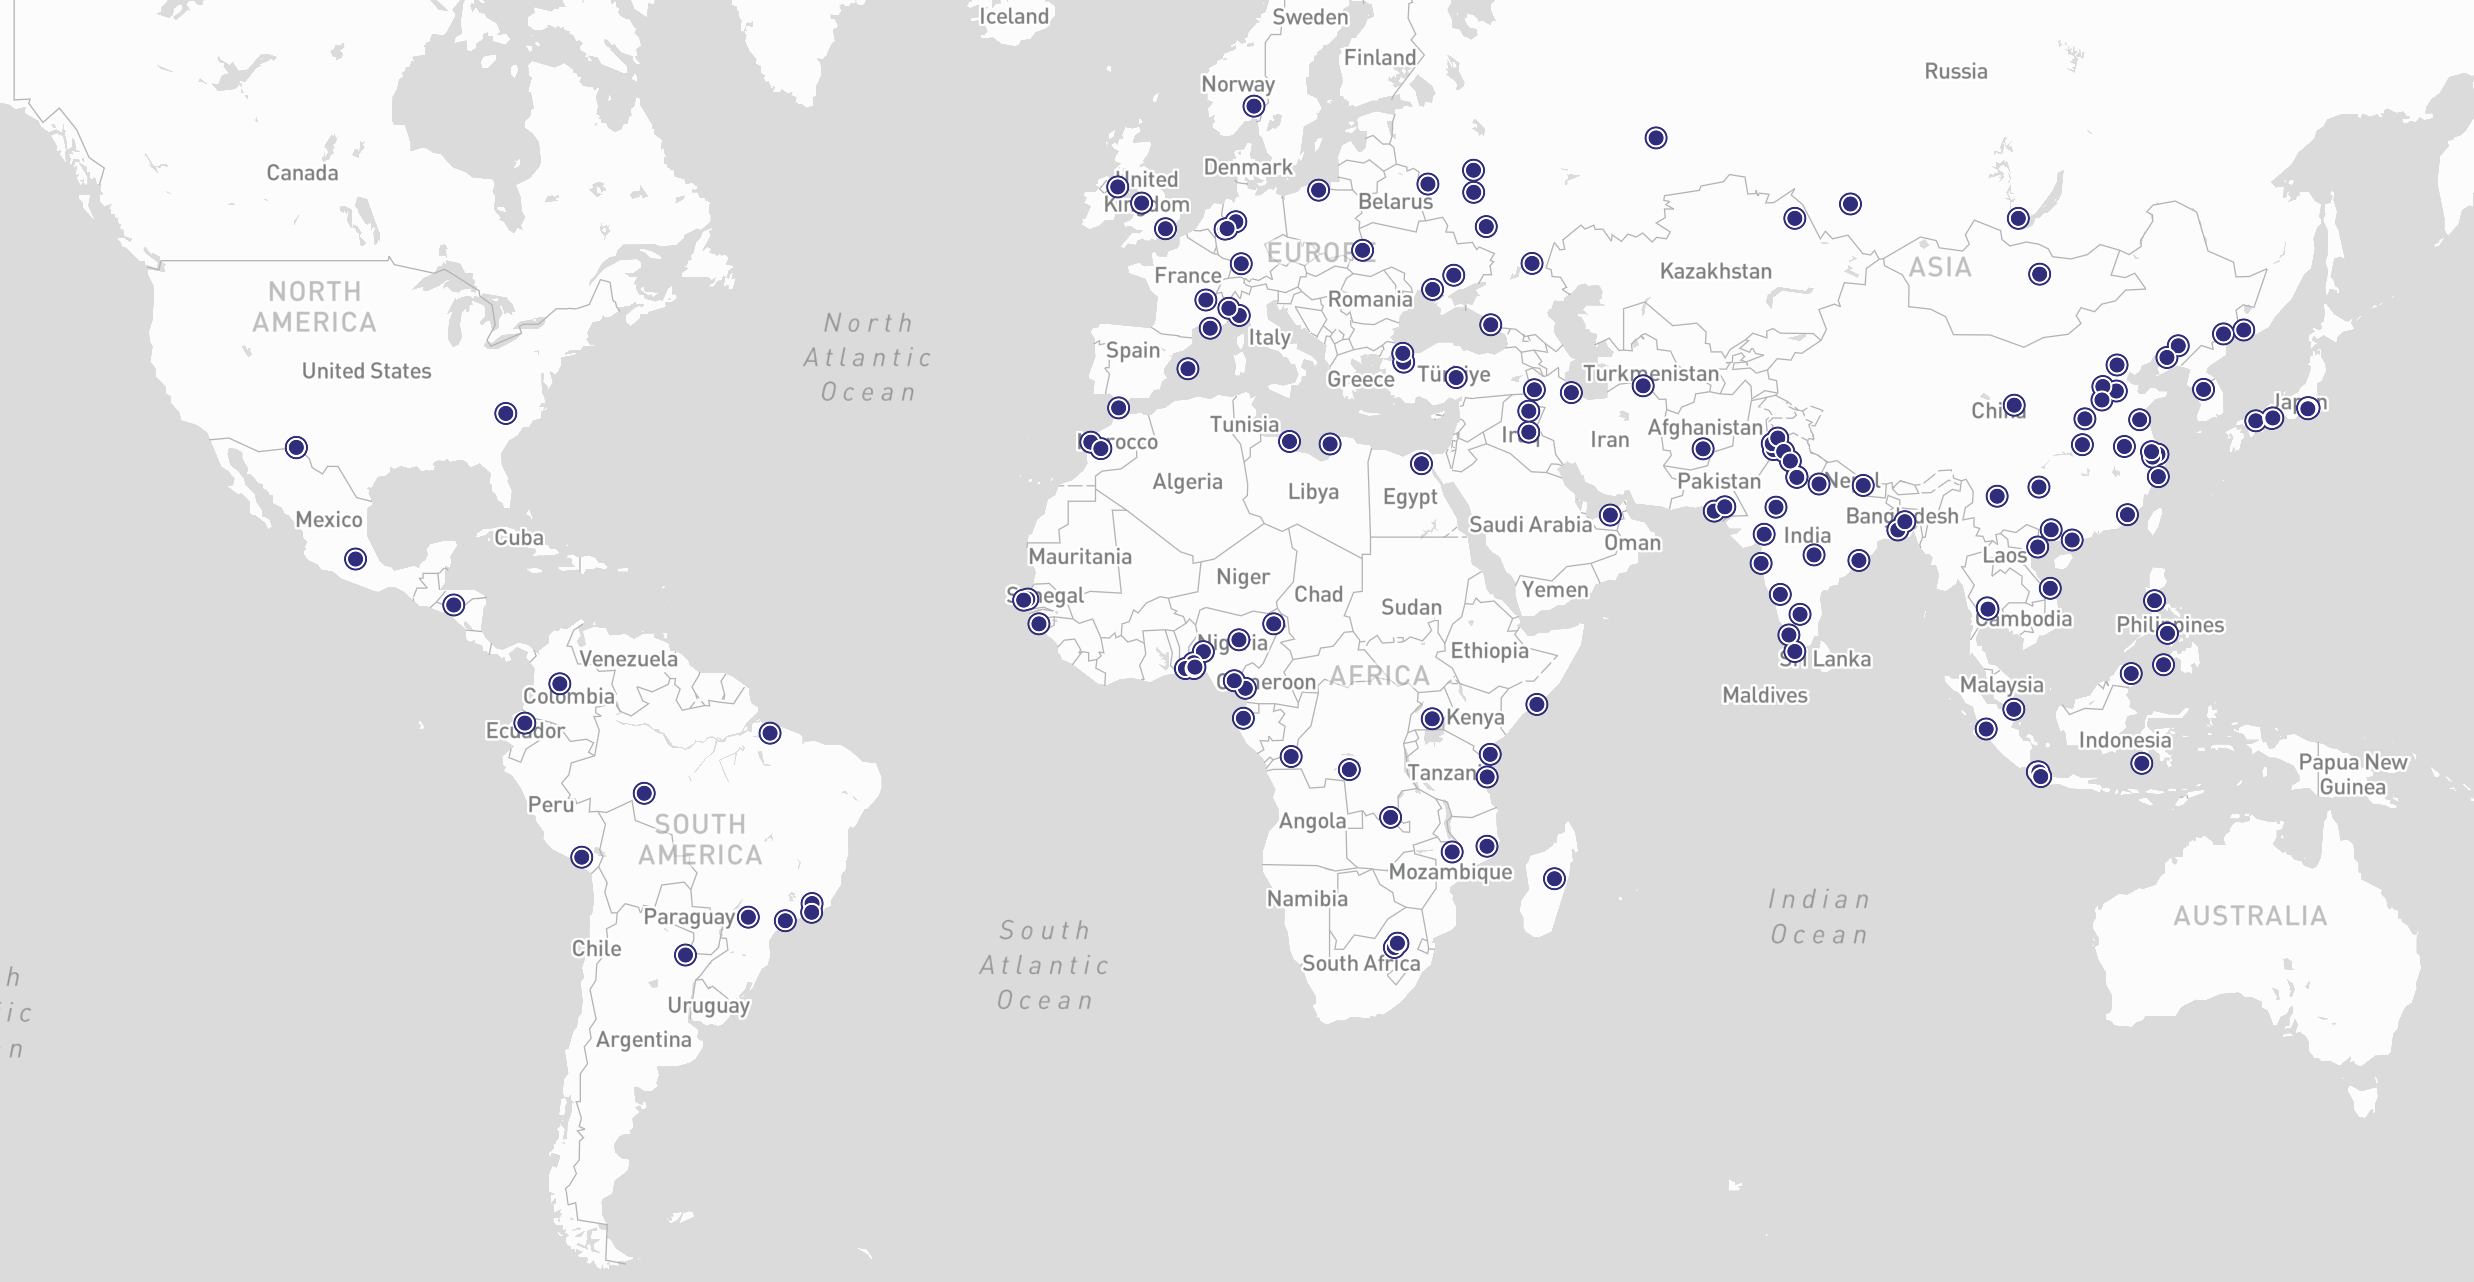
\includegraphics[width=\linewidth]{figures/150puntos.png}
    \caption{150 ciudades en el mapa}
    \label{fig:mapa150}
\end{figure}

\subsection*{Etapa 1}
En la primera etapa no se tenía el módulo automatizado para las pruebas, por lo que la afinación
de los hiperparámetros se realizó de forma manual y empírica. Durante esta fase temprana se
ejecutaron las primeras 15,000 iteraciones manteniendo los parámetros constantes y variando
únicamente la semilla. El índice de soluciones factibles rondaba en el $7\%$ y la mejor solución
encontrada evaluaba a 0.15001. Es probable que los lotes fueran demasiado pequeños, por una
corazonada incorrecta se eligió un tamaño de 500, muy lejos del óptimo final que rondaba los 4000.

\subsection*{Etapa 2}
El inicio de la segunda etapa lo marcó la implementación del módulo de experimentación, fue un 
punto de inflexión en el proyecto, ya que permitió automatizar y escalar significativamente el
volumen de pruebas concurrentes, además de brindar un mayor control y
registro sistemático de los resultados. \\

Tras evaluar 60,000 semillas con variaciones ligeras en los hiperparámetros, se alcanzó una
solución con una función de costo de 0.143194 con la siguiente configuración de parámetros:

\begin{verbatim}
    -seed 3259
    -targetP 0.9
    -epsilonP 0.00001
    -initialT 8
    -tempSample 5000
    -coolingFactor 0.95
    -epsilon 0.00001
    -batchSize 5000
    -maxAttempts 150
\end{verbatim}

Con estos argumentos, se obtuvo la siguiente ruta:

\begin{figure}[htbp]
    \centering
    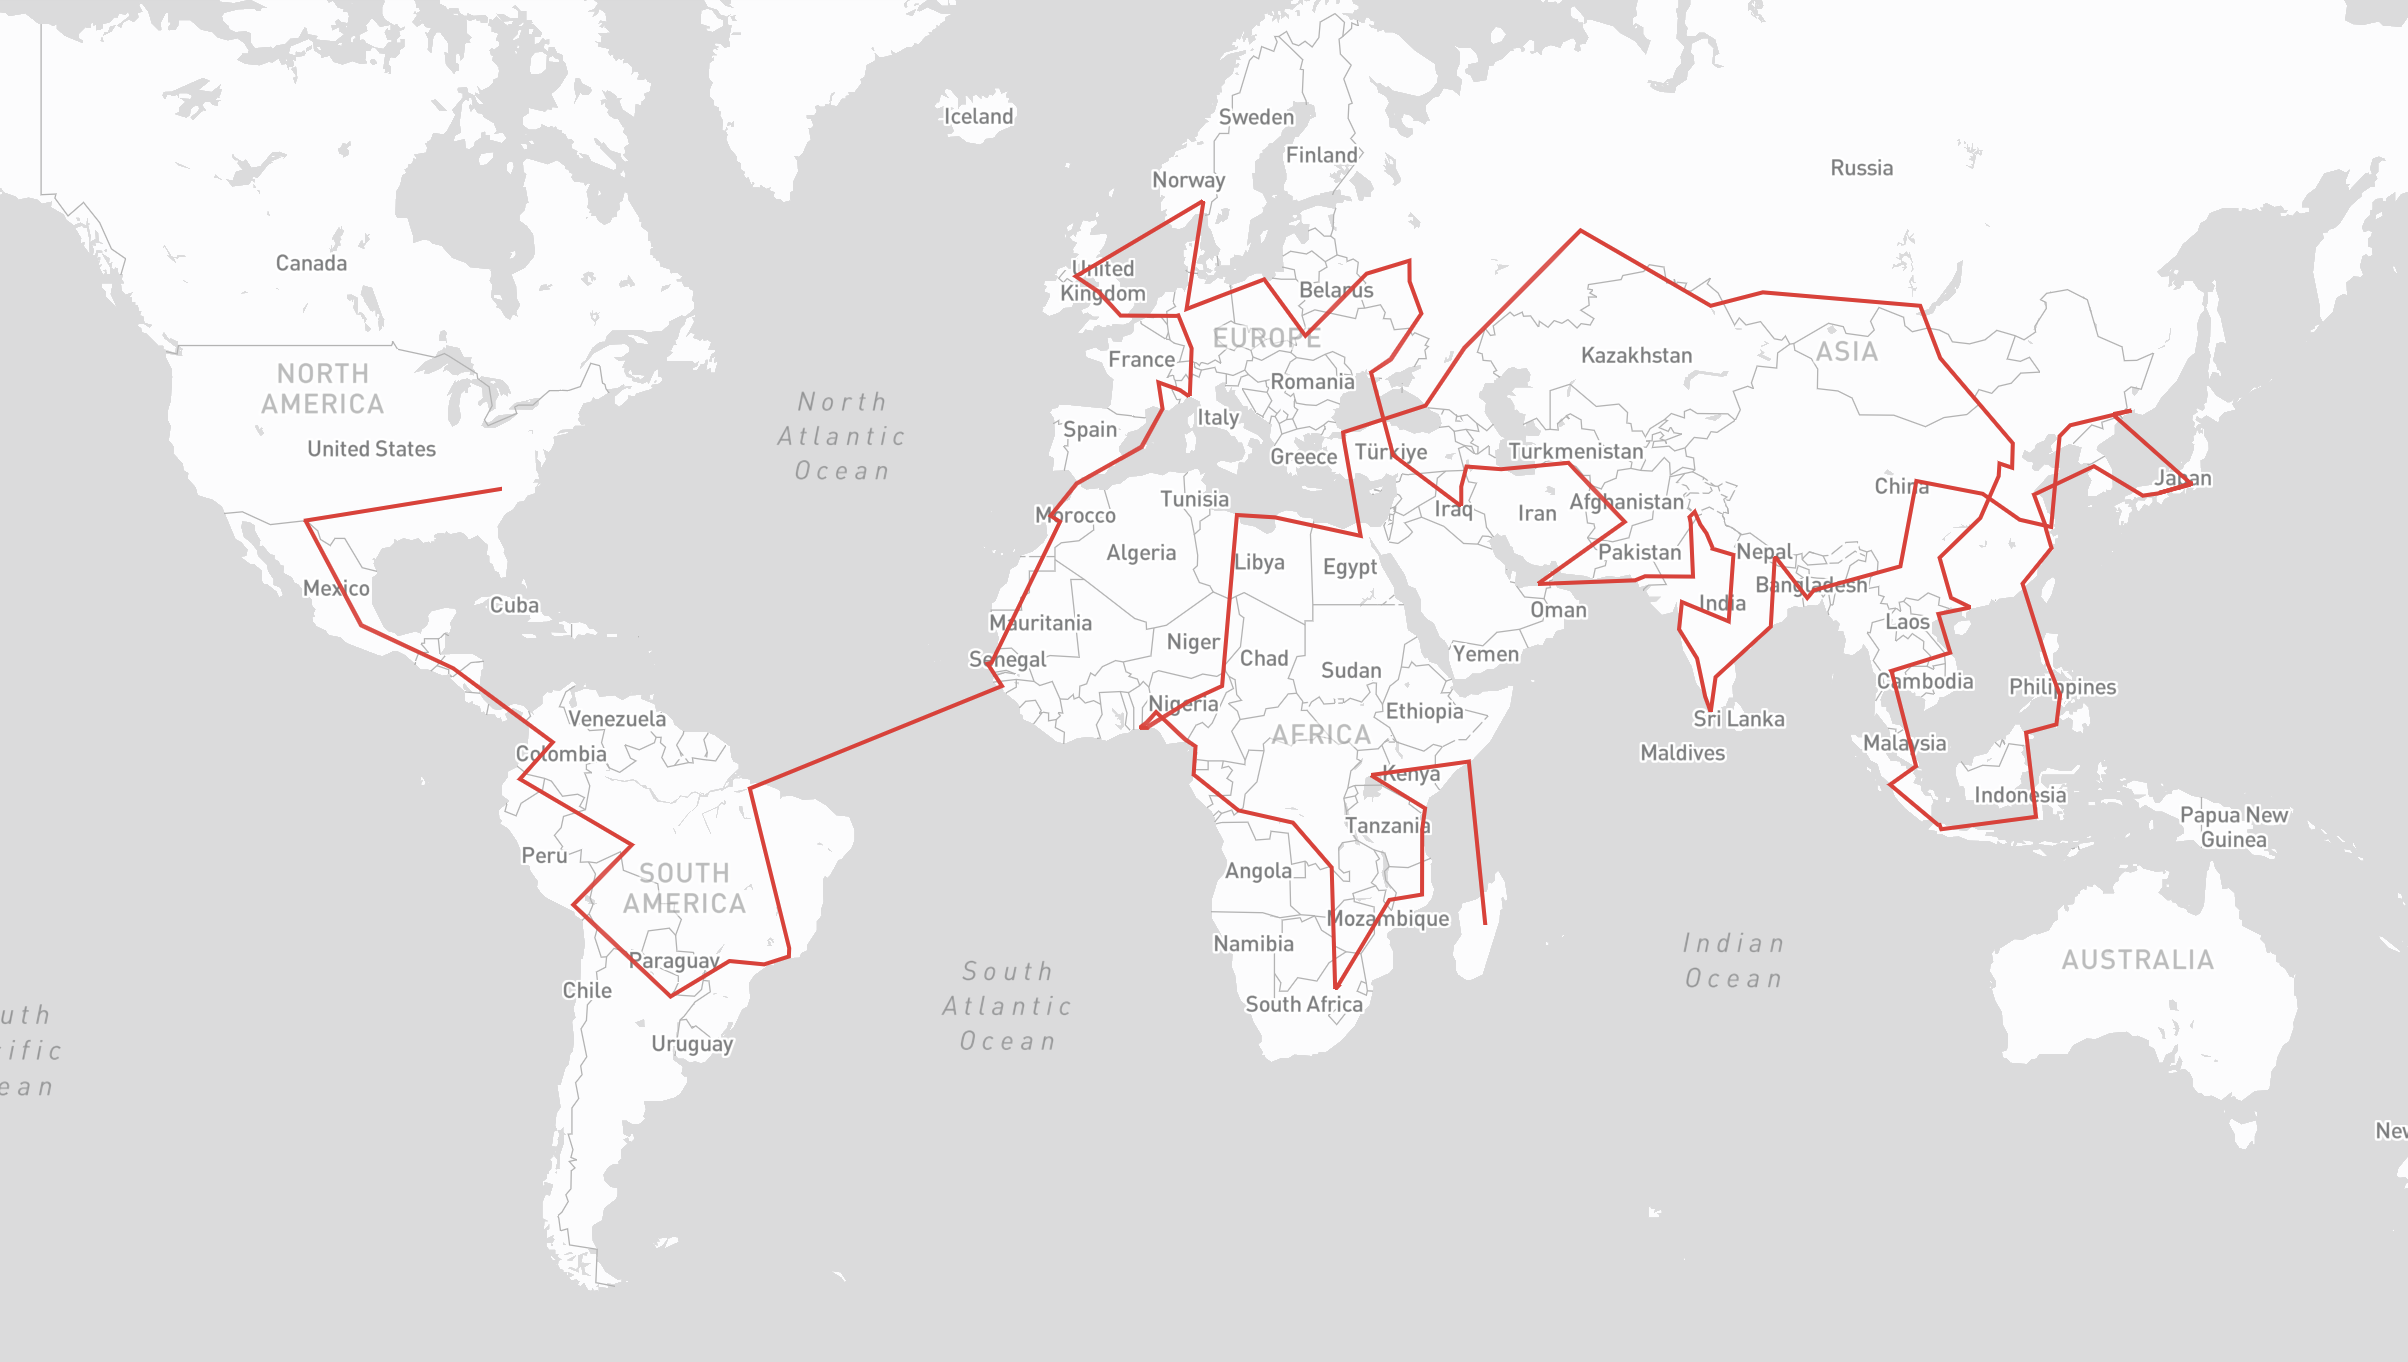
\includegraphics[width=\linewidth]{figures/Sol150_map_1.png}
    \caption{Ruta de costo 0.143194 para tsp 150.}
    \label{fig:mapa150_sol_1}
\end{figure}

\begin{quote}
    171, 77, 183, 346, 75, 821, 512, 483, 1075, 652, 179, 671, 16, 520, 186, 675, 340, 502, 828, 12, 1038, 339, 244, 826, 444, 17, 164, 11, 984, 995, 837, 979, 493, 509, 329, 19, 839, 496, 182, 673, 665, 344, 653, 490, 654, 26, 820, 345, 332, 181, 14, 982, 187, 816, 678, 823, 7, 507, 656, 667, 184, 815, 9, 832, 661, 663, 657, 829, 1, 986, 508, 168, 505, 2, 173, 172, 163, 676, 22, 185, 351, 991, 27, 353, 990, 333, 3, 165, 981, 1004, 6, 5, 978, 352, 668, 176, 23, 988, 174, 4, 489, 817, 347, 499, 491, 492, 25, 501, 1003, 349, 331, 662, 8, 999, 334, 674, 985, 343, 510, 660, 20, 825, 500, 504, 511, 327, 670, 350, 840, 336, 980, 297, 1001, 74, 822, 166, 658, 666, 818, 655, 819, 330, 1073, 169, 1037, 326, 328, 167, 495, 494 
\end{quote}

Este proceso involucró la evaluación de más de 3 millones de soluciones potenciales. La
siguiente gráfica corresponde a la temperatura de aceptación a lo largo de dicha ejecución:

\begin{figure}[htbp]
    \centering
    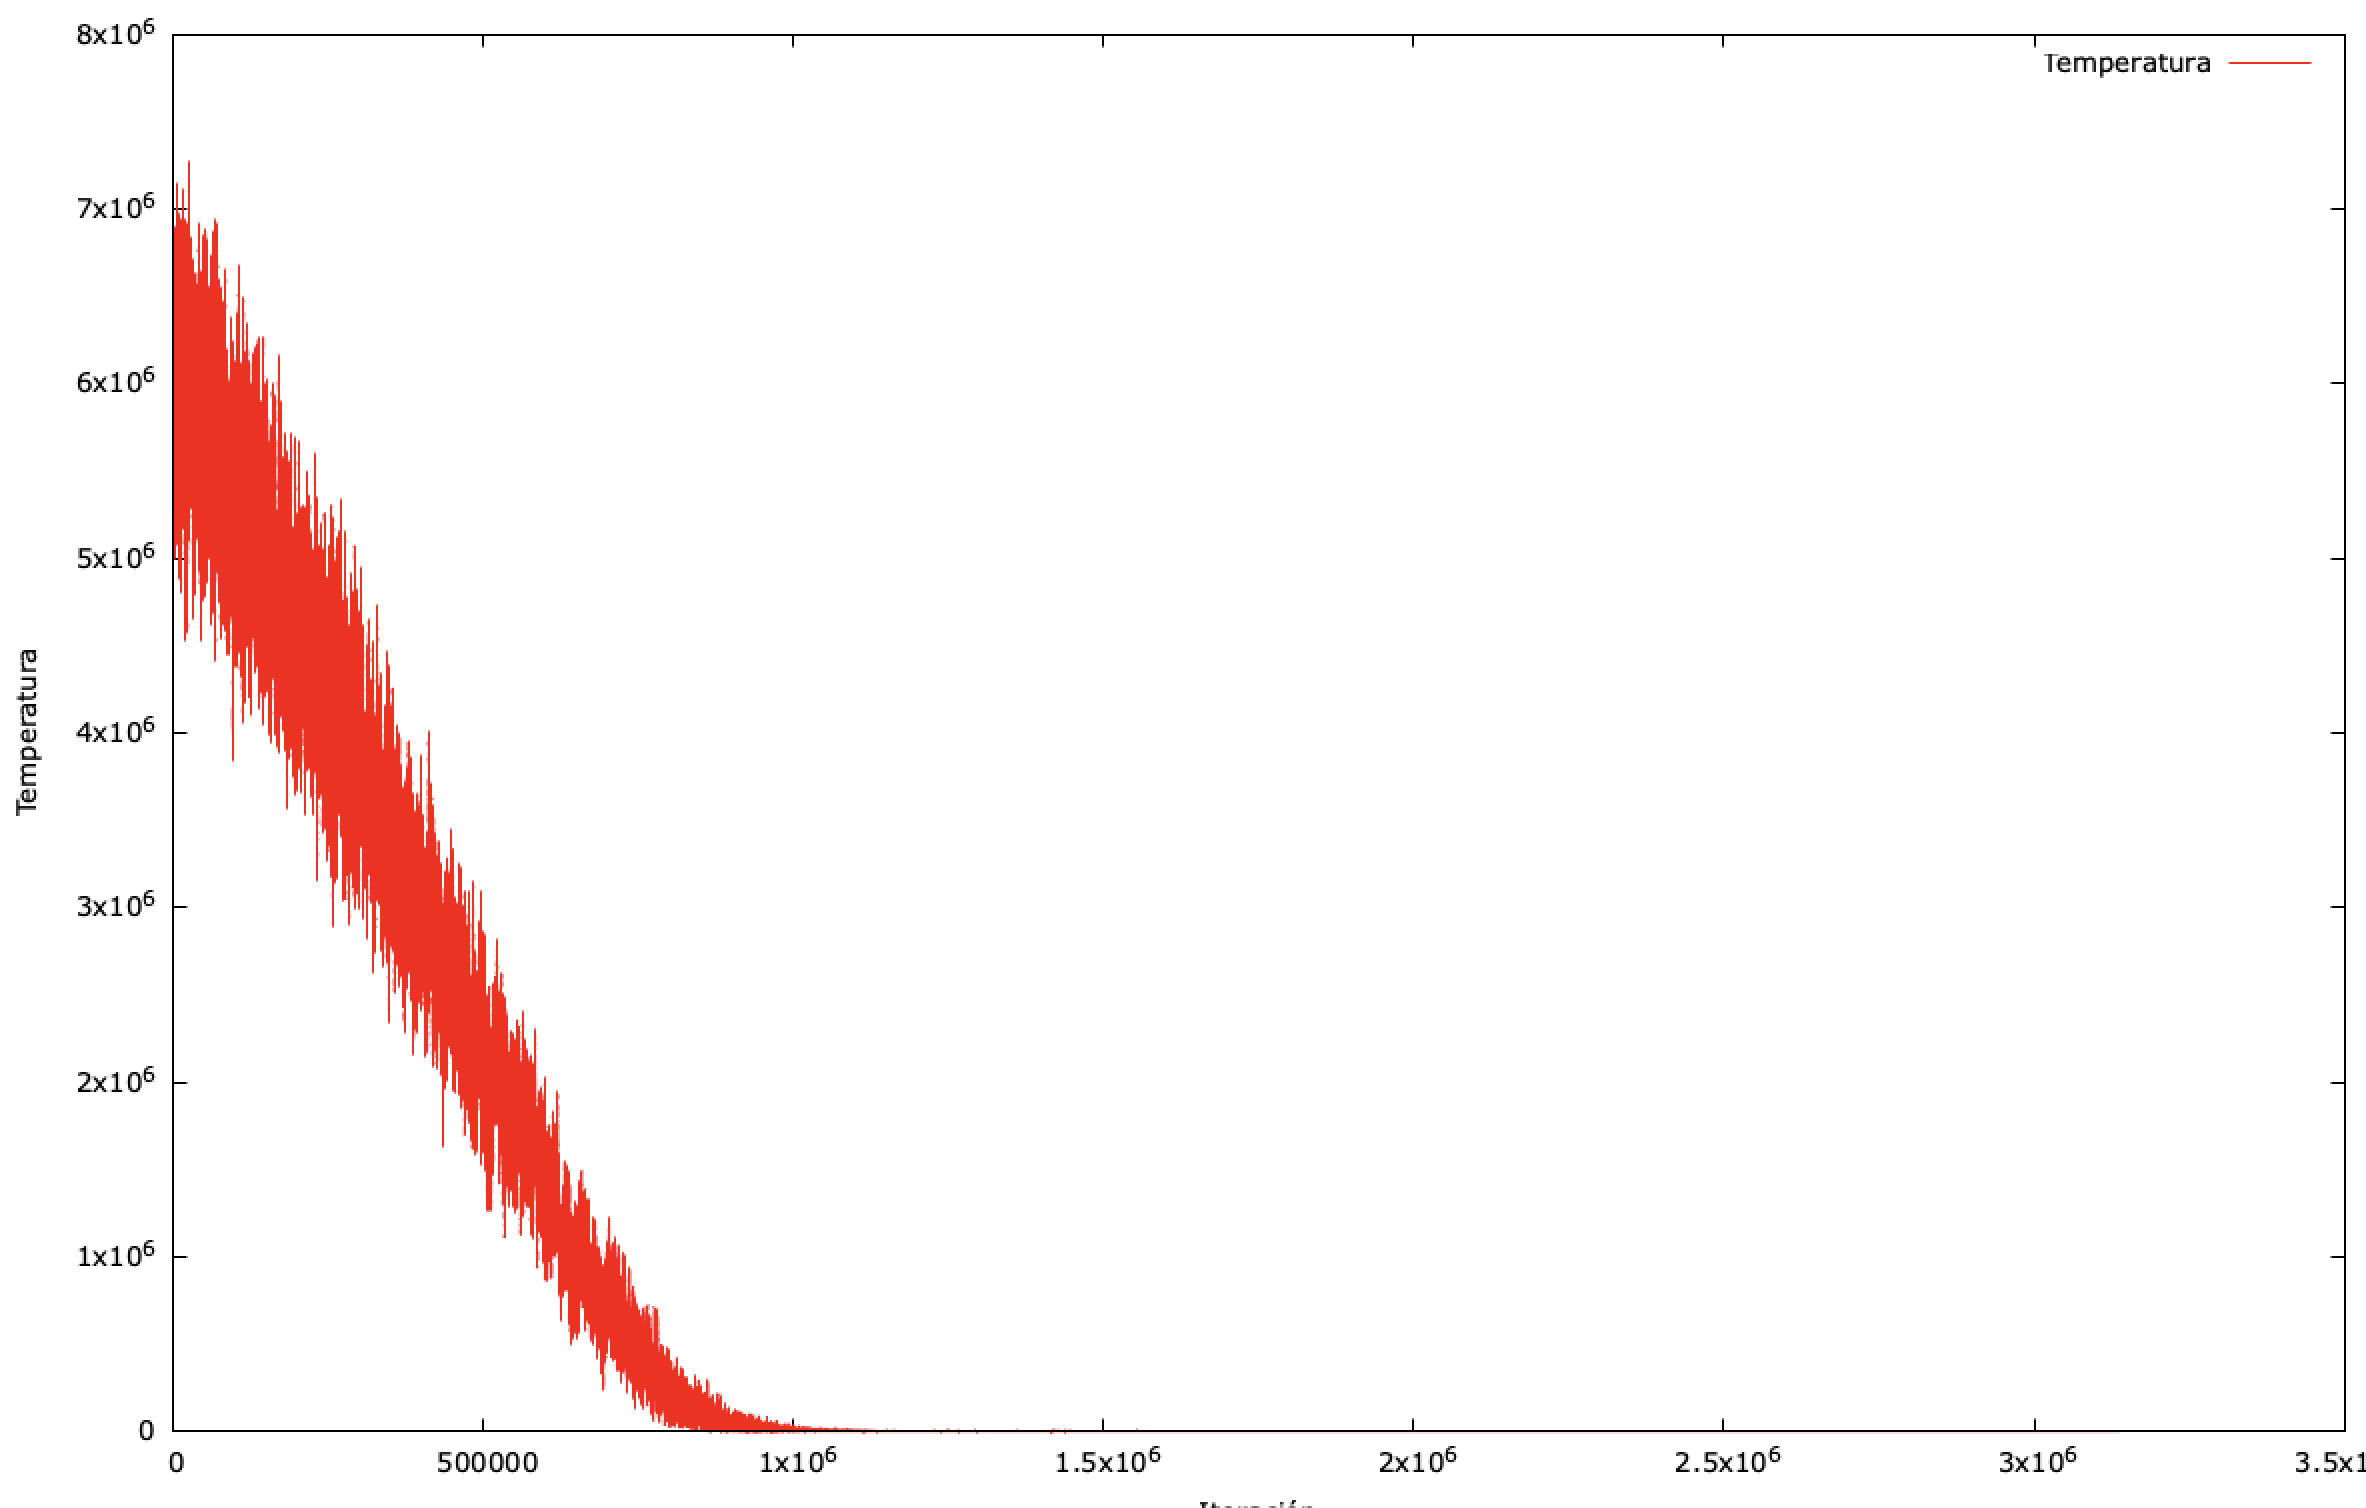
\includegraphics[width=\linewidth]{figures/acep150_1.png}
    \caption{Evolución de la función de costo con respecto a la aceptación.}
    \label{fig:temp1}
\end{figure}
No obstante, de las 60,000 semillas evaluadas, la mejor solución se obtuvo con el número 3259,
mientras que las 56,741 restantes no lograron superar dicho resultado.

\subsection*{Etapa 3}
Lo que marcó la transición de la segunda a la tercera etapa de experimentación fue la modificación 
del modelo, particularmente, la generación de la vecindad. Inicialmente el sistema implementó de forma
estricta la definición planteada en la asignatura, generando vecinos mediante el intercambio de
dos ciudades elegidas al azar. Con este modelo, el sistema tendía a estancarse en valores 0.14
para la instancia de 150 ciudades. Al realizar un análisis comparativo entre la mejor solución
obtenida hasta ese momento por este proyecto (0.143) y los resultados del resto del grupo
(0.140), se observó que el intercambio necesario para igualar las soluciones necesitaba invertir
el orden de un segmento completo e intercambiar dos ciudades. Bajo el esquema que se tenía
resultaba casi imposible, ya que cada cambio destruye hasta cuatro aristas dentro de la gráfica,
lo que rompe la estructura global del recorrido y reduce la probabilidad de conservar aristas
óptimas. Para mitigar este problema, se sustituyó el operador por inversión de subarreglos,
\textit{2-opt}, similar a la propuesta original de Kirkpatrick.~\cite{kirkpatrick1983}. \\

Con este nuevo enfoque, al seleccionar dos índices aleatorios \(i\) y \(j\), en lugar de
intercambiar únicamente las ciudades en esas posiciones, se invierte el segmento intermedio que
las conecta. Esto solo altera a lo más dos aristas del recorrido total. La implementación fue
notable, permitió al algoritmo descender a valores inferiores a 0.14. \\

Además de este cambio, en la tercera etapa se implementó una generación aleatoria para los
hiperparámetros dentro de rangos acotados, mismos que fueron seleccionados en relación a los argumentos
que funcionaban para la primera y segunda etapa. Tras varias pruebas, se determinó empíricamente que no
resultaba conveniente variar la condición de paro del algoritmo ($\epsilon$) ni los parámetros de la
heurística de temperatura inicial, entonces estos valores se mantuvieron constantes: 
$\epsilon = 0.00001$, $\epsilon_P = 0.00001$ y una temperatura inicial de $T_0 = 8$. \\

Los hiperparámetros que sí variaron se obtuvieron a partir de distribuciones uniformes aleatorias en
los siguientes rangos:
\begin{itemize}
    \item Probabilidad objetivo (targetP): entre $0.7000$ y $0.9500$.
    \item Factor de enfriamiento (coolingFactor): entre $0.8500$ y $0.9800$.
    \item Tamaño del lote (batchSize): entre $1000$ y $5000$.
    \item Muestra de temperatura (tempSample): entre $1000$ y $5000$.
    \item Intentos máximos (maxAttempts): entre $50$ y $200$.
\end{itemize}

Con esto, el sistema logró generar un \(100\%\) de soluciones factibles y alcanzar un costo de 0.13624,
el cual representa el mejor resultado registrado en todo el proyecto. Más aún, esta solución no se
obtuvo de manera aislada, sino que fue recurrente entre el \(10\%\) y el \(15\%\) de las ejecuciones.  \\

En la Tabla~\ref{tab:resultados_exp} se presentan 17 semillas distintas que lograron converger
exactamente a la misma solución con el costo mínimo de 0.13624. Algunas ejecuciones arrojaron la misma
ruta pero en orden inverso.

\begin{table*}[htbp]
    \centering
    \caption{Parámetros y resultados ordenados por tiempo de ejecución}
    \label{tab:resultados_exp}
    \footnotesize
    \begin{tabular}{|l|c|c|c|c|c|c|c|c|c|c|c|}
        \hline
        \textbf{label} & \textbf{seed} & \textbf{targetP} & \textbf{initialT} & \textbf{tempSample} & \textbf{cooling} & \textbf{batch} & \textbf{maxAtt} & \textbf{initialCost} & \textbf{finalCost} & \textbf{ms} \\ \hline
        \texttt{exp\_3\_307} & 6331 & 0.7176 & 8 & 4289 & 0.8626 & 2698 & 71 & 6343092.5 & 0.13624 & 1324 \\ \hline
        \texttt{exp\_3\_291} & 6176 & 0.8648 & 8 & 1163 & 0.9050 & 1325 & 127 & 6221527.1 & 0.13624 & 2688 \\ \hline
        \texttt{exp\_3\_109} & 4356 & 0.8424 & 8 & 4340 & 0.9339 & 3261 & 86 & 7275850.9 & 0.13624 & 2998 \\ \hline
        \texttt{exp\_3\_293} & 6192 & 0.7402 & 8 & 3206 & 0.8899 & 1754 & 161 & 6574041.2 & 0.13624 & 3469 \\ \hline
        \texttt{exp\_3\_413} & 7392 & 0.7341 & 8 & 2486 & 0.9359 & 2132 & 84 & 6736284.7 & 0.13624 & 3637 \\ \hline
        \texttt{exp\_3\_451} & 7778 & 0.9195 & 8 & 4537 & 0.8996 & 2127 & 136 & 6940206.6 & 0.13624 & 3672 \\ \hline
        \texttt{exp\_3\_323} & 6492 & 0.8863 & 8 & 2078 & 0.9131 & 4253 & 98 & 6623070.3 & 0.13624 & 3817 \\ \hline
        \texttt{exp\_3\_158} & 4842 & 0.8548 & 8 & 3987 & 0.9175 & 2961 & 109 & 7283770.1 & 0.13624 & 4711 \\ \hline
        \texttt{exp\_3\_371} & 6978 & 0.9213 & 8 & 4787 & 0.9280 & 2161 & 165 & 6651777.1 & 0.13624 & 5227 \\ \hline
        \texttt{exp\_3\_367} & 6929 & 0.7844 & 8 & 1265 & 0.8777 & 3716 & 192 & 7103496.4 & 0.13624 & 5622 \\ \hline
        \texttt{exp\_3\_240} & 5664 & 0.7614 & 8 & 1102 & 0.9383 & 2329 & 119 & 6774678.8 & 0.13624 & 5690 \\ \hline
        \texttt{exp\_3\_176} & 5026 & 0.8955 & 8 & 3029 & 0.9261 & 2512 & 166 & 7662501.5 & 0.13624 & 6348 \\ \hline
        \texttt{exp\_3\_197} & 5229 & 0.7065 & 8 & 3659 & 0.9216 & 3758 & 158 & 6479806.5 & 0.13624 & 7528 \\ \hline
        \texttt{exp\_3\_712} & 3971 & 0.9224 & 8 & 4561 & 0.9380 & 3139 & 133 & 6638076.8 & 0.13624 & 7568 \\ \hline
        \texttt{exp\_3\_249} & 5756 & 0.9158 & 8 & 1361 & 0.9630 & 3115 & 194 & 7469804.6 & 0.13624 & 13022 \\ \hline
        \texttt{exp\_3\_181} & 5076 & 0.8246 & 8 & 2261 & 0.9693 & 2876 & 164 & 6781088.0 & 0.13624 & 13949 \\ \hline
        \texttt{exp\_3\_219} & 5452 & 0.9100 & 8 & 1004 & 0.9694 & 4849 & 172 & 6818784.3 & 0.13624 & 20392 \\ \hline
    \end{tabular}
\end{table*}

El mapa de la solución y la secuencia de los identificadores de la respuesta de costo 0.13624 es
la siguiente:
\begin{figure}[htbp]
    \centering
    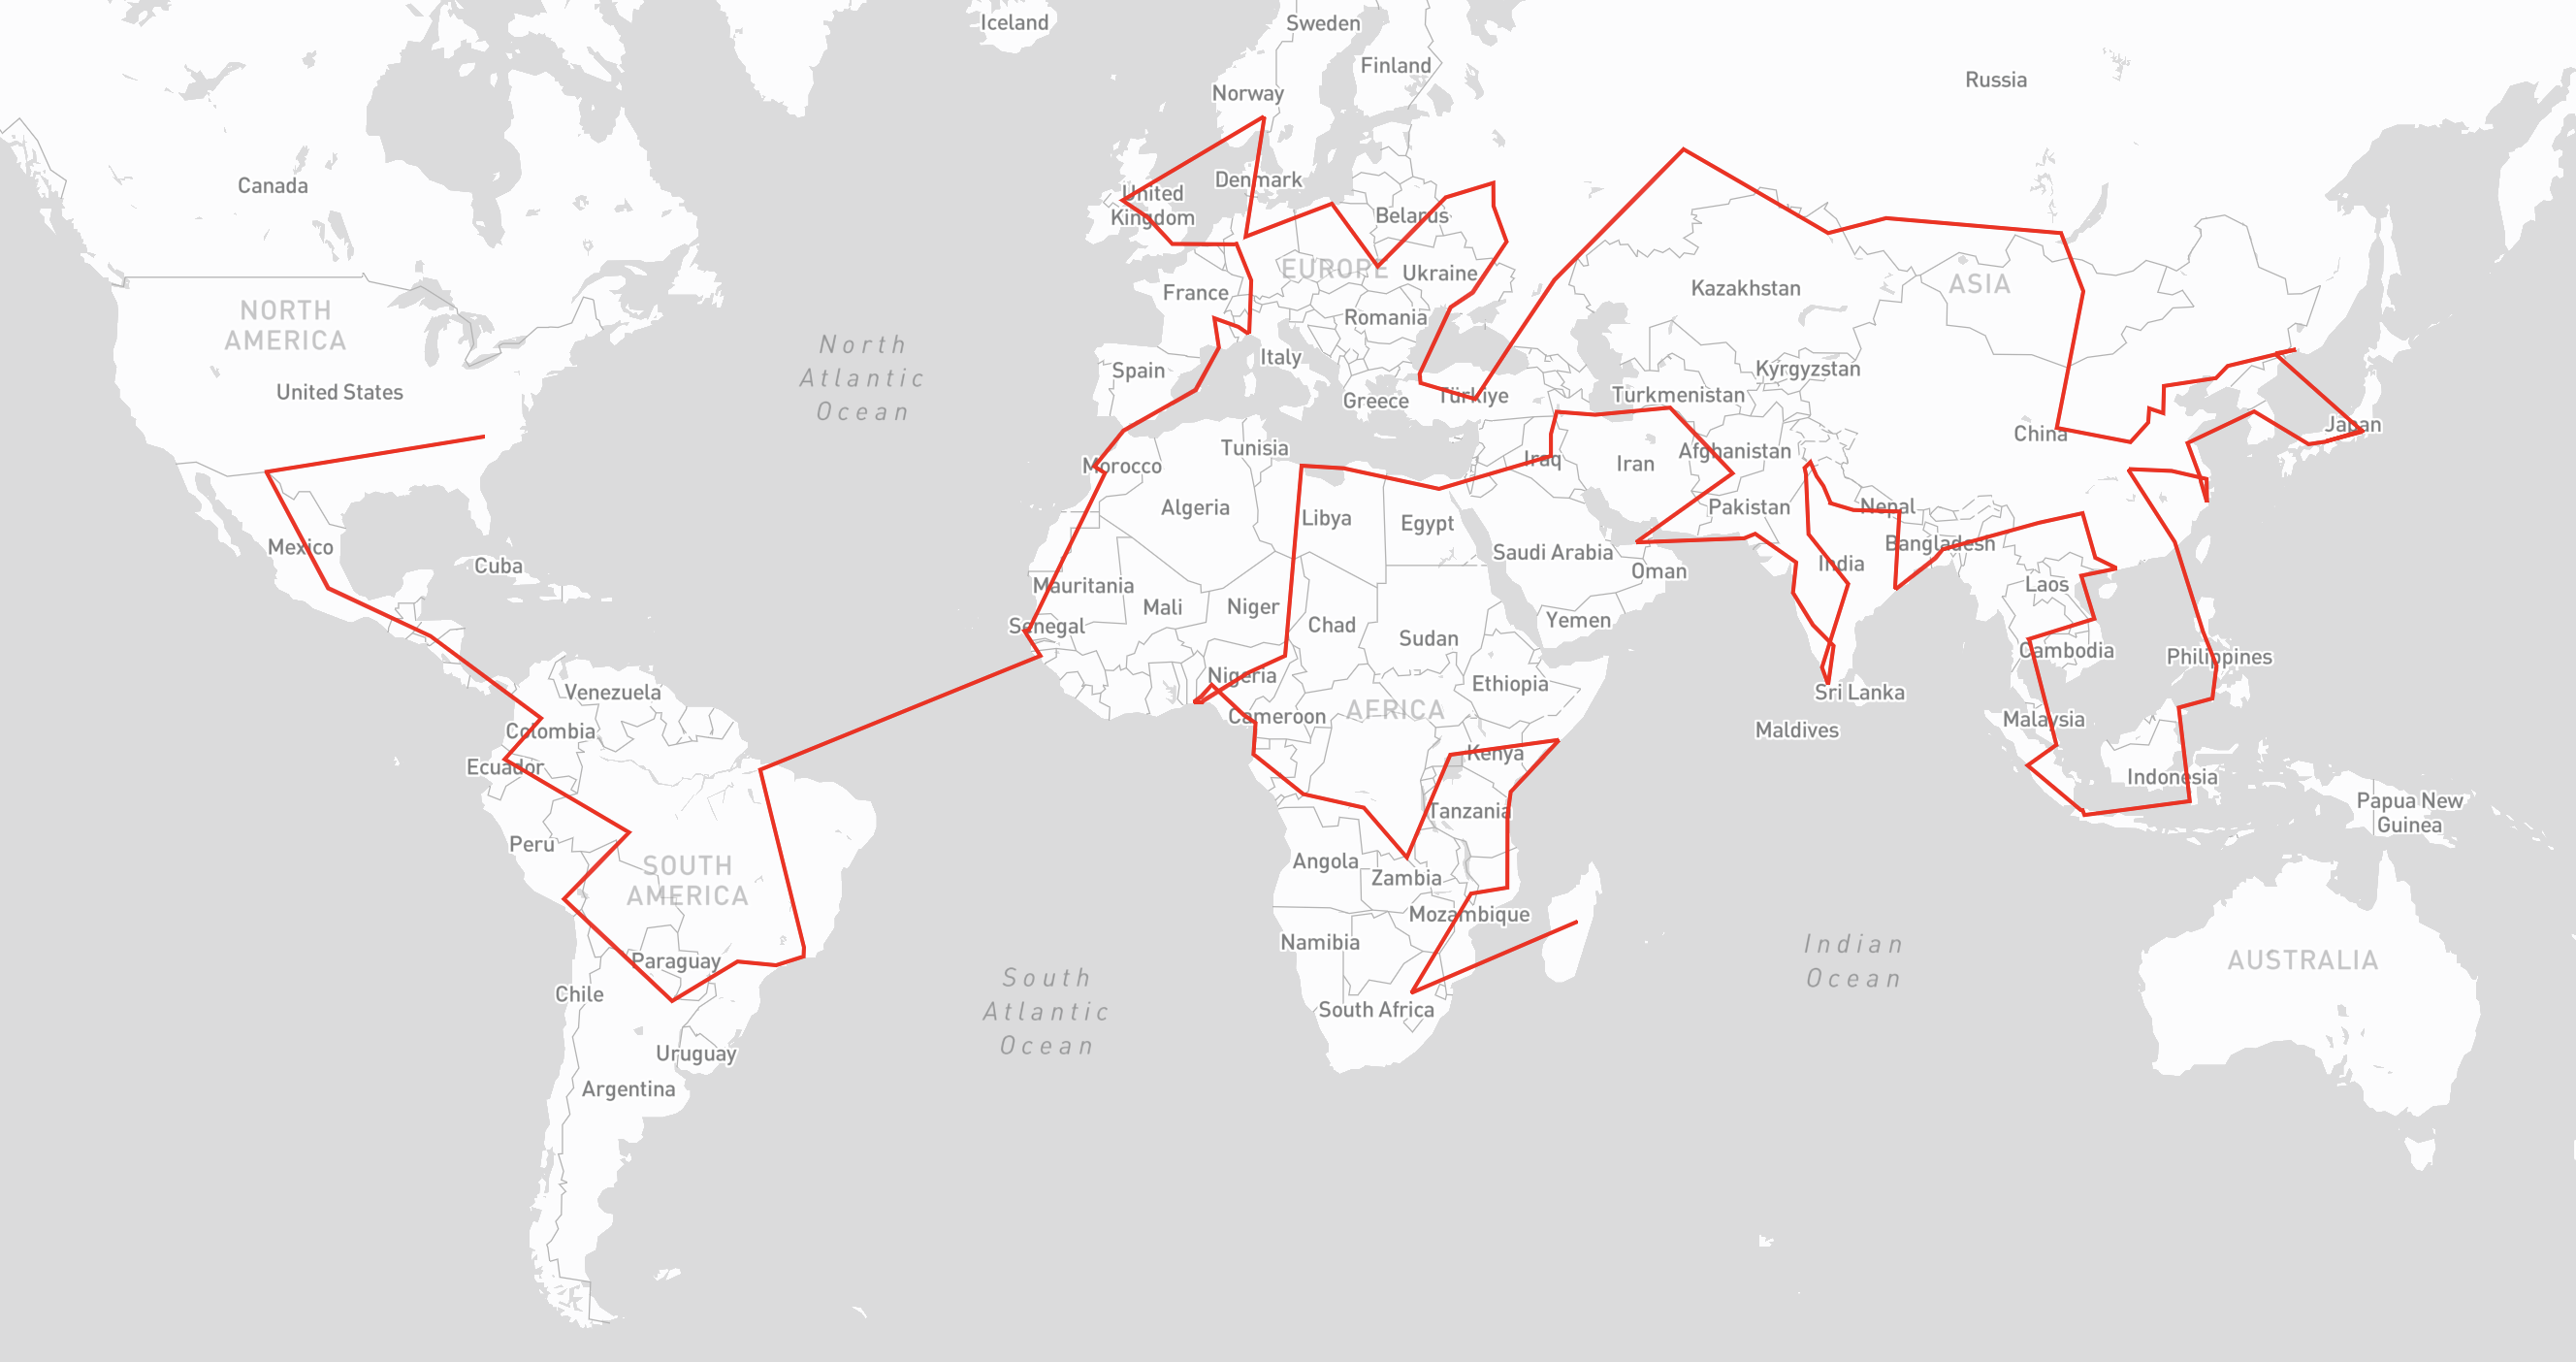
\includegraphics[width=\linewidth]{figures/Sol150_map_2.png}
    \caption{Ruta final obtenida por el algoritmo de Recocido Simulado para la instancia de 150 ciudades de costo 0.13624}
    \label{fig:mapa150_sol}
\end{figure}

\begin{quote}
171, 652, 1075, 483, 512, 821, 75, 346, 77, 183, 179, 671, 16, 520, 186, 675, 340, 502, 828, 12, 1038, 339, 244, 826, 444, 17, 25, 492, 491, 499, 347, 817, 489, 4, 174, 165, 3, 333, 27, 353, 990, 981, 988, 23, 176, 668, 352, 978, 5, 6, 1004, 351, 991, 185, 22, 676, 665, 344, 653, 490, 654, 26, 820, 345, 332, 181, 14, 982, 187, 816, 678, 823, 7, 507, 673, 173, 2, 656, 667, 184, 815, 9, 832, 661, 663, 657, 829, 1, 986, 508, 168, 505, 19, 839, 496, 182, 172, 163, 329, 509, 493, 979, 837, 995, 984, 501, 164, 11, 1003, 349, 331, 662, 8, 999, 334, 674, 985, 343, 510, 660, 20, 825, 500, 504, 511, 327, 670, 350, 840, 336, 980, 297, 1001, 74, 822, 166, 658, 666, 818, 655, 819, 330, 1073, 169, 1037, 326, 328, 167, 495, 494.
\end{quote}

Si bien todos los experimentos en la Tabla~\ref{tab:resultados_exp} llegan exactamente a la misma
solución, el tiempo de cómputo requerido difiere significativamente entre ellos. Por ejemplo,
tomando los experimentos etiquetados como \texttt{exp\_3\_176} y \texttt{exp\_3\_219}, el primero alcanza
la convergencia con aproximadamente 1 millón de evaluaciones y el segundo requiere cerca de 3 millones.

Esto se ve en las Figuras~\ref{fig:acep1} y~\ref{fig:acep2}, aun cuando la escala dificulta apreciar
esta diferencia.\\

Parámetros del \texttt{exp\_3\_176}:
\begin{verbatim}
    -seed 5026
    -targetP 0.8955
    -epsilonP 0.00001
    -initialT 8
    -tempSample 3029
    -coolingFactor 0.9261
    -epsilon 0.00001
    -batchSize 2512
    -maxAttempts 166
\end{verbatim}

\begin{figure}[htbp]
    \centering
    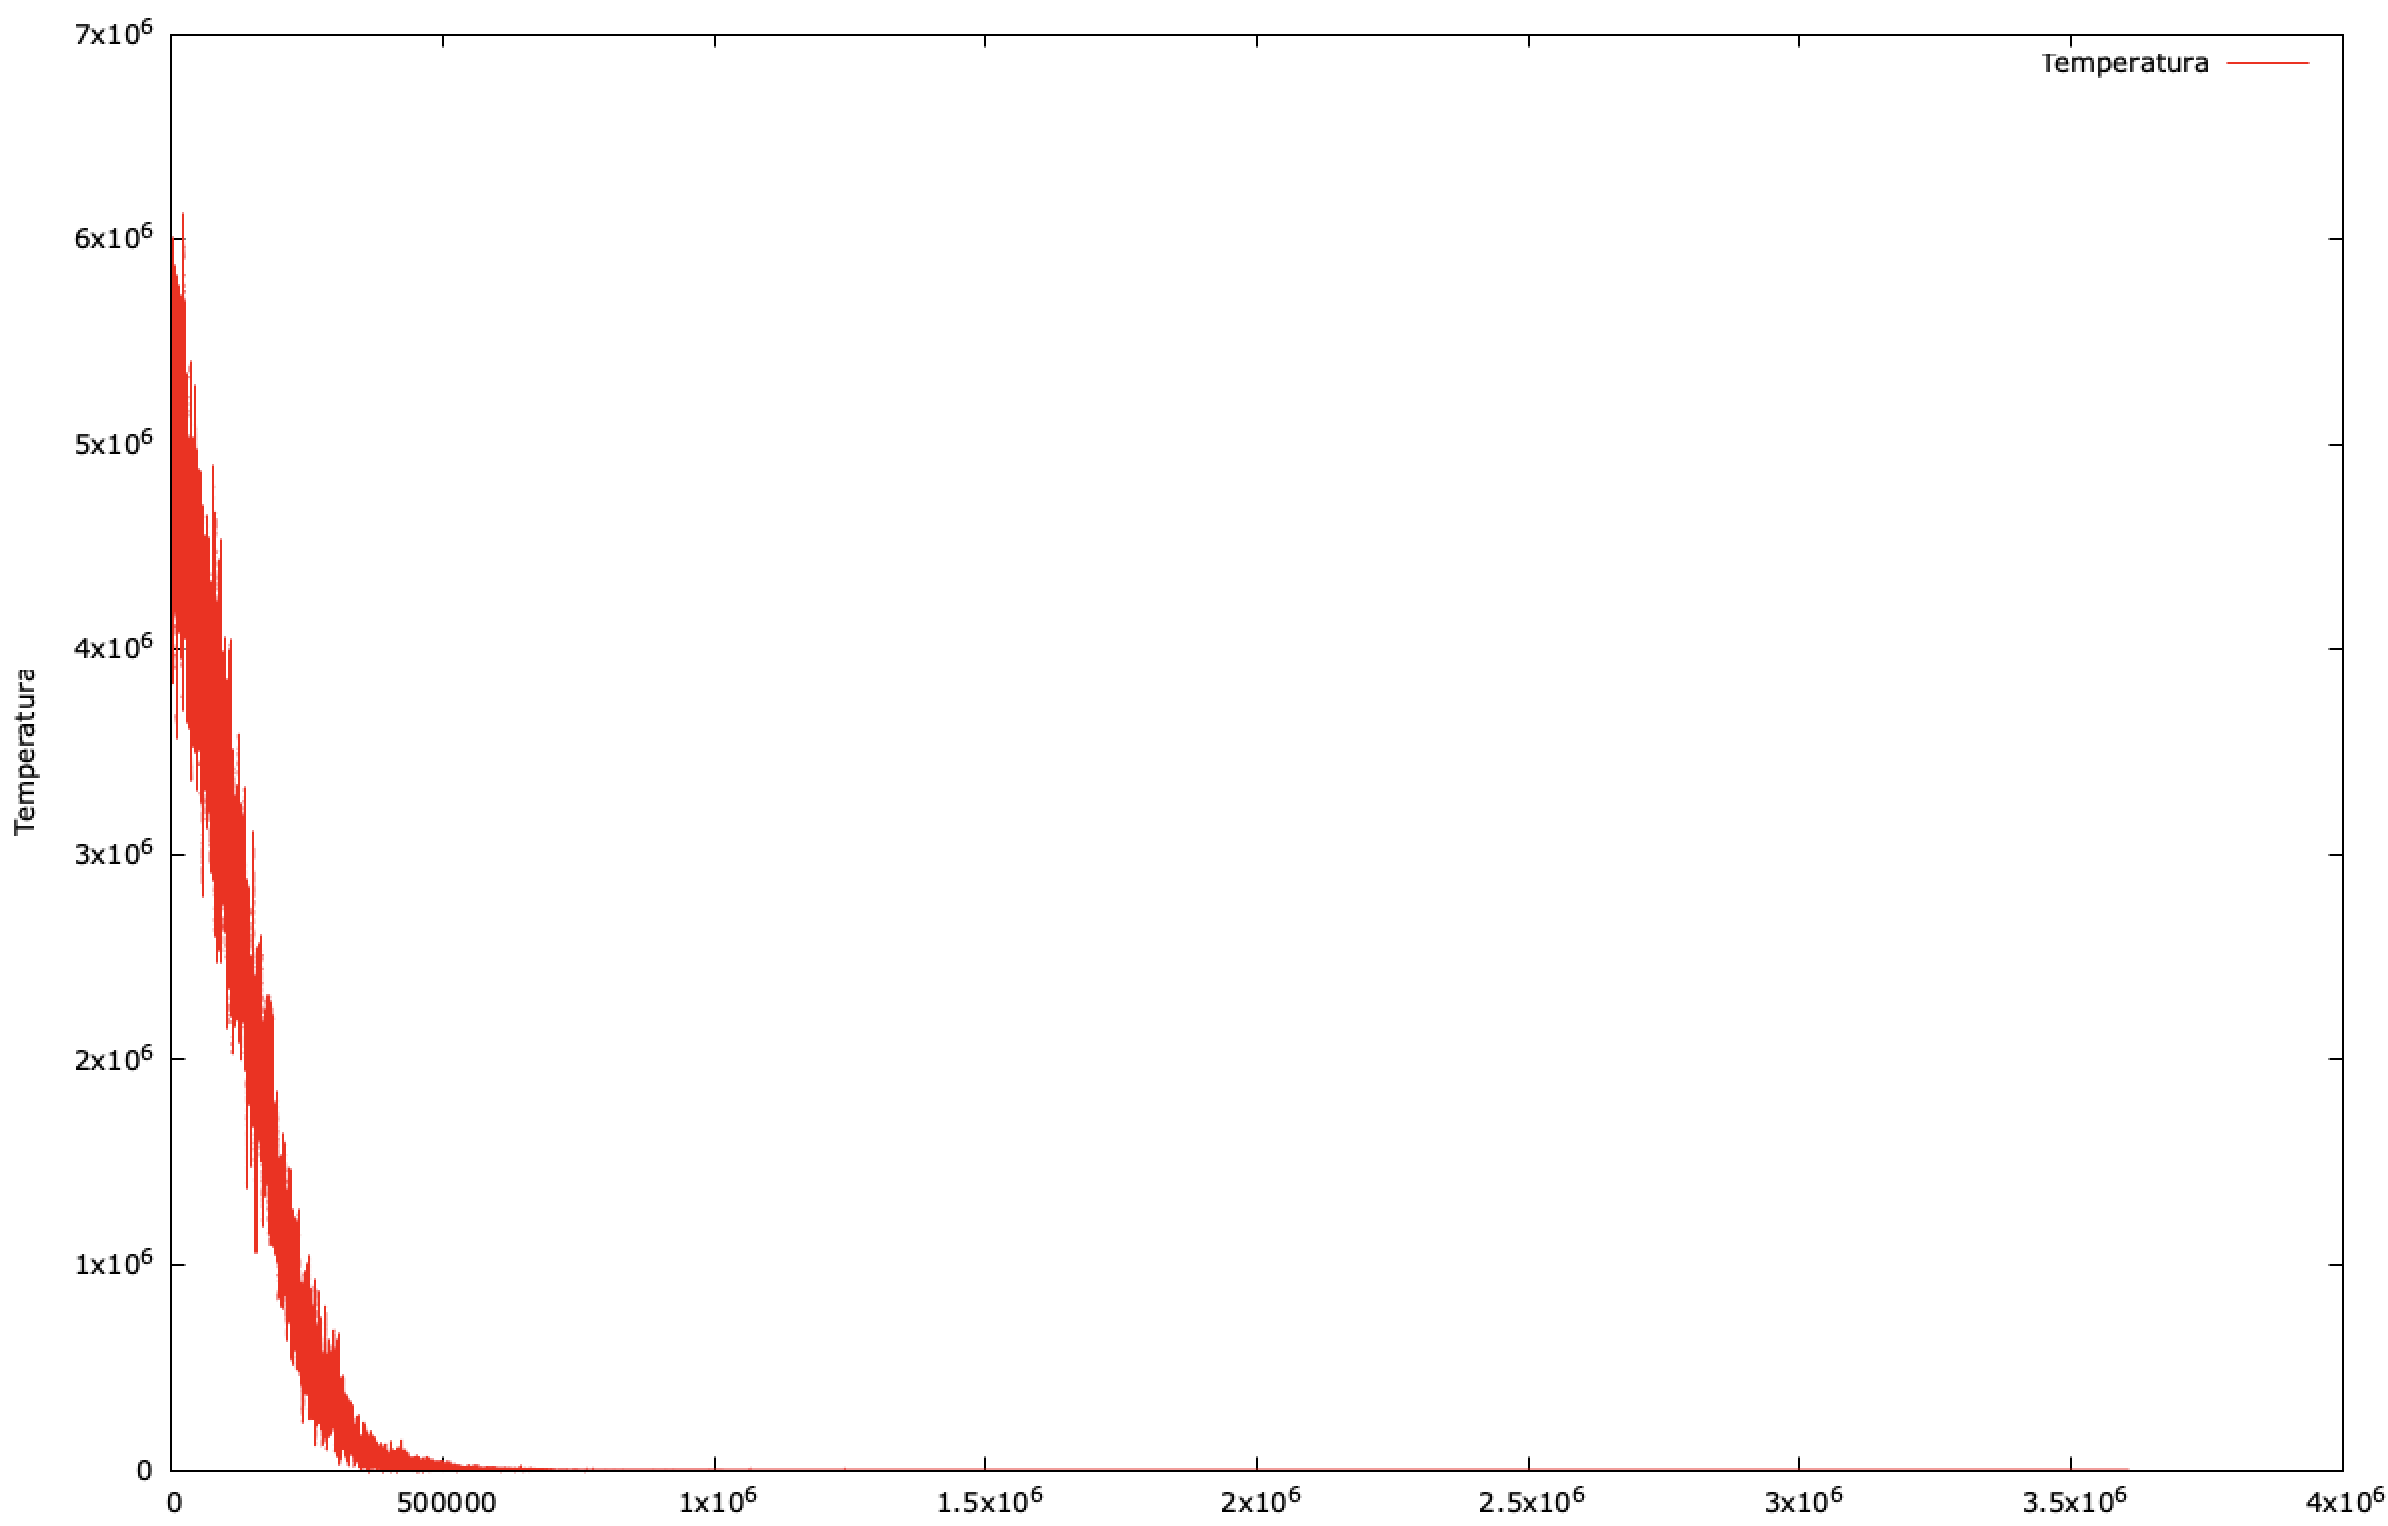
\includegraphics[width=\linewidth]{figures/acep150_2.png}
    \caption{Evolución de la función de costo con respecto a la temperatura en la ejecución \texttt{exp\_3\_176} }
    \label{fig:acep1}
\end{figure}

Parámetros del \texttt{exp\_3\_219}:
\begin{verbatim}
    -seed 5452
    -targetP 0.91
    -epsilonP 0.00001
    -initialT 8
    -tempSample 1004
    -coolingFactor 0.9694
    -epsilon 0.00001
    -batchSize 4849
    -maxAttempts 172
\end{verbatim}

\begin{figure}[htbp]
    \centering
    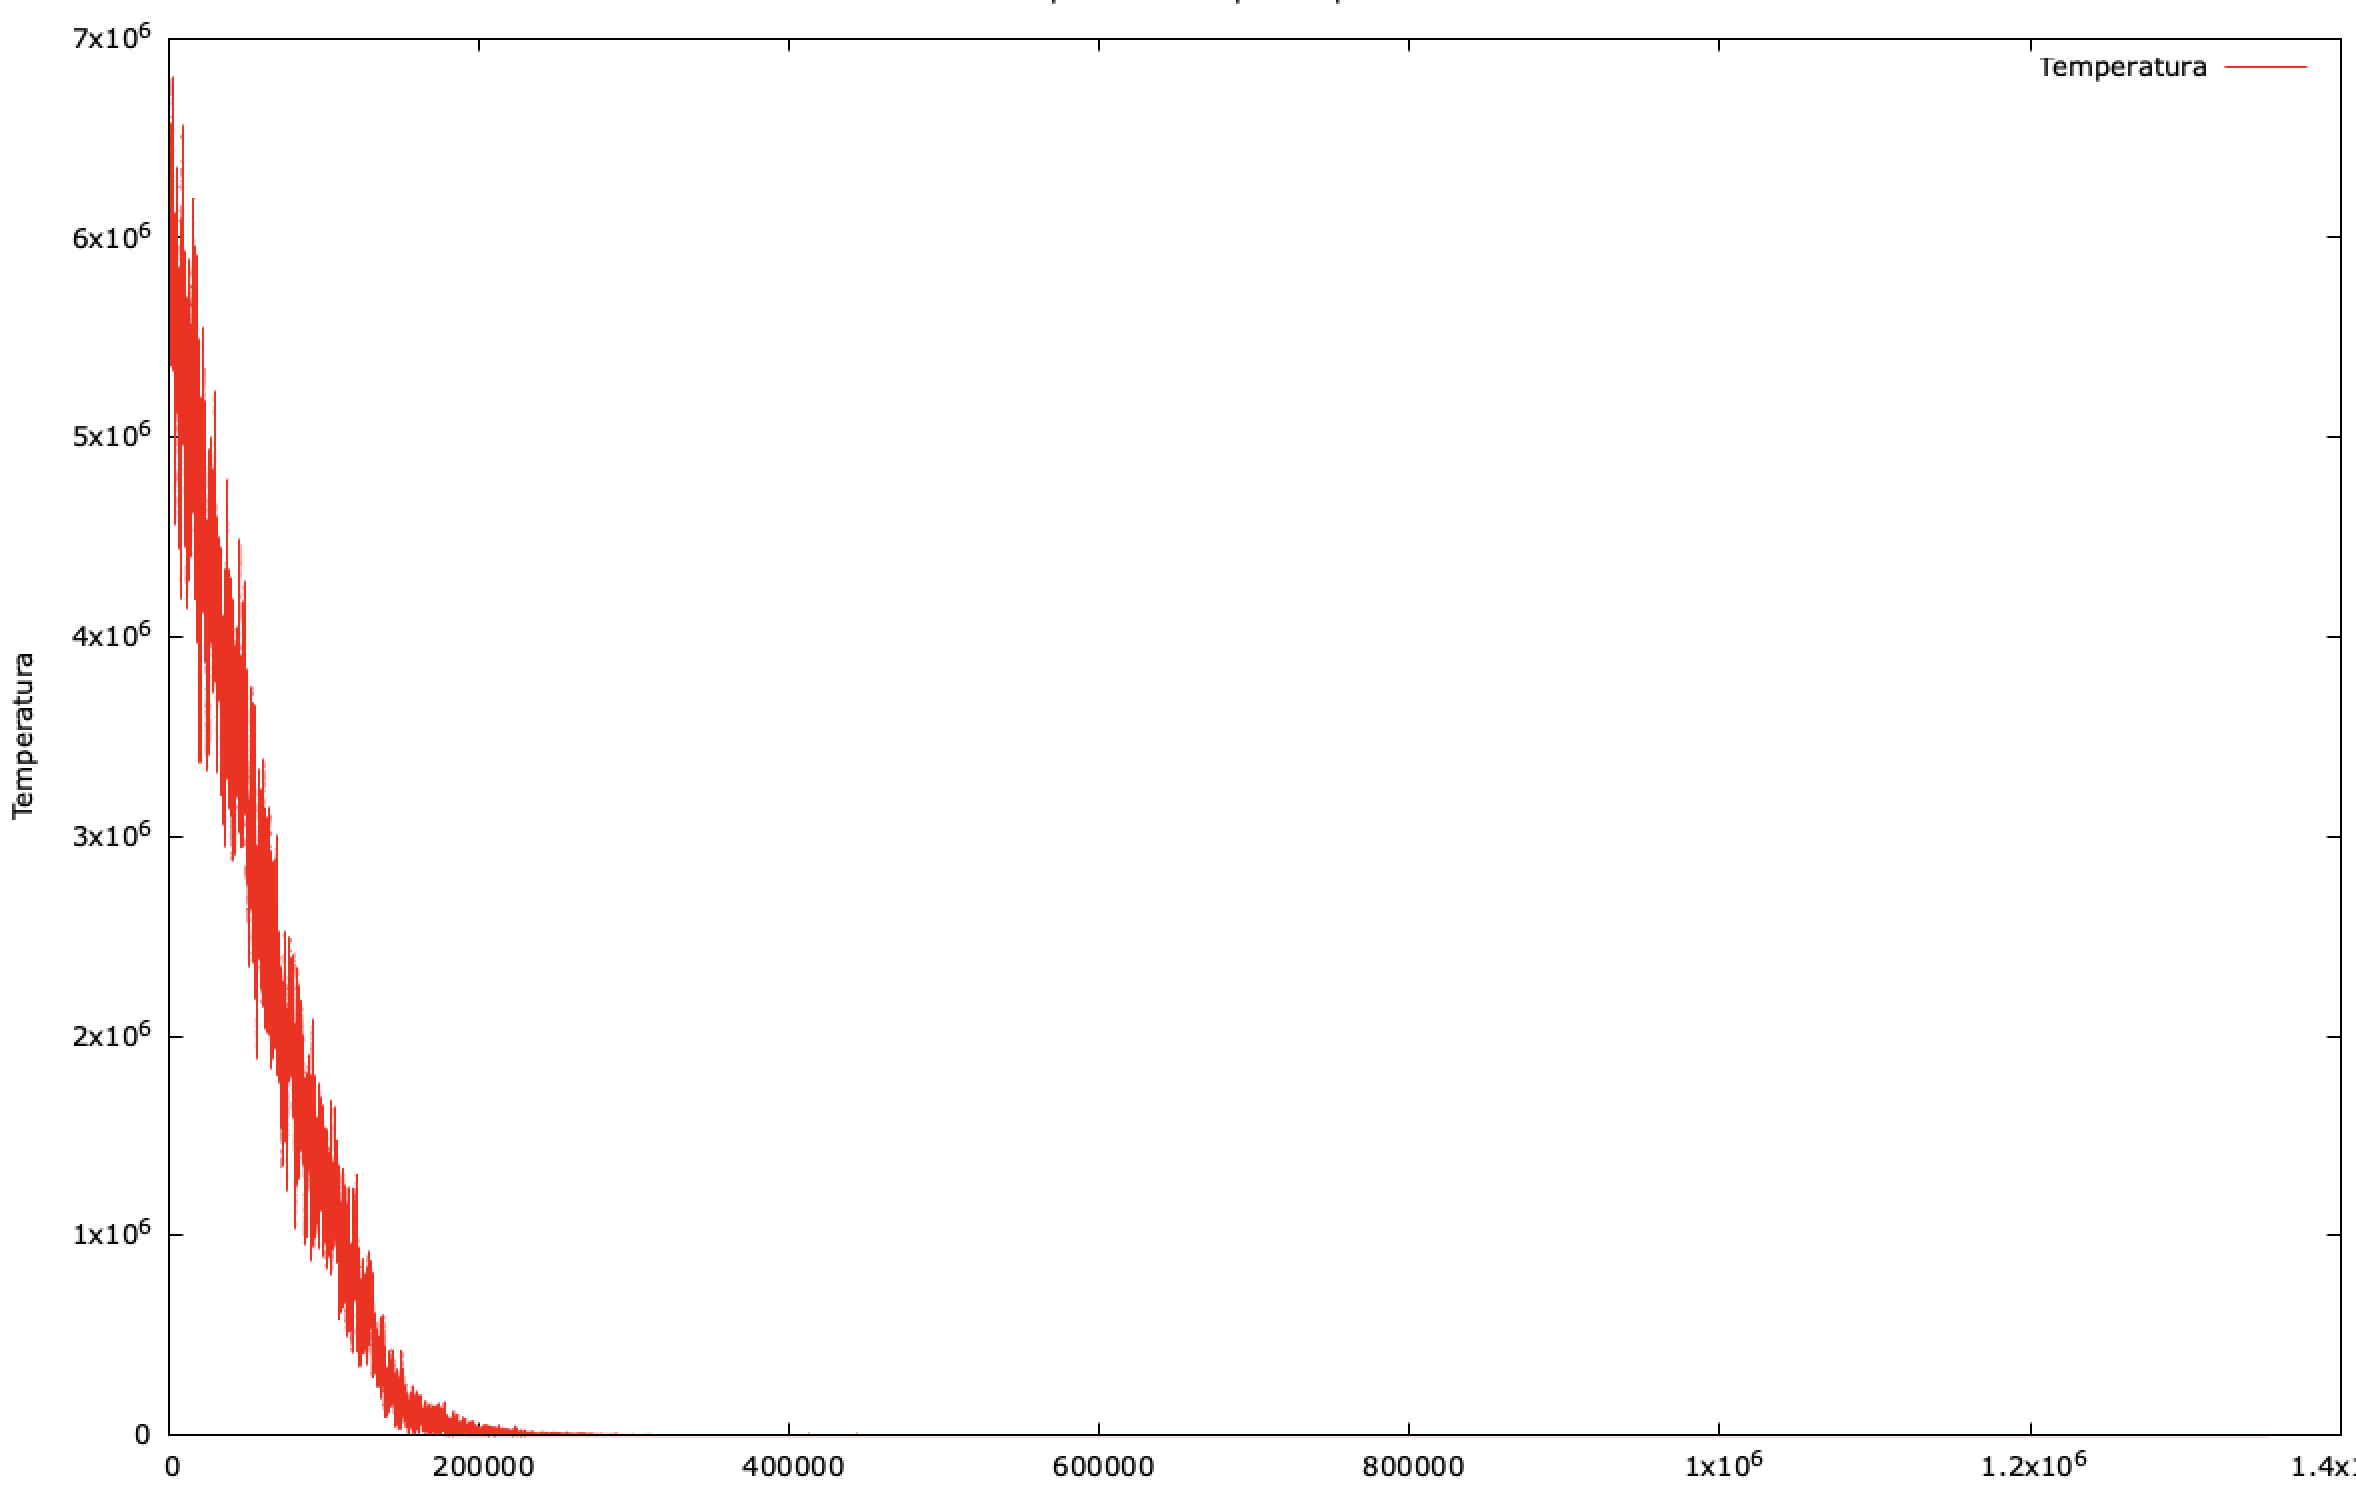
\includegraphics[width=\linewidth]{figures/acept150_3.png}
    \caption{Evolución de la función de costo con respecto a la temperatura en la ejecución \texttt{exp\_3\_219}}
    \label{fig:acep2}
\end{figure}

\subsection*{Hiperparámetros promedio}
A partir de un conjunto de 5,000 ejecuciones con parámetros aleatorios, se trató de calcular el
promedio aritmético de las configuraciones evaluadas con el fin de definir un estándar. Los valores
promedio obtenidos, tomando una entrada de $n$ ciudades, son:
\begin{itemize}
    \item Probabilidad objetivo (targetP): $0.8247$
    \item Factor de enfriamiento (coolingFactor): $0.9149$
    \item Muestra de temperatura (tempSample): $19.85 * n$
    \item Tamaño del lote (batch): $19.94 * n$
    \item Intentos máximos (maxAttempts): $0.83 * n$
\end{itemize}

Para validar estas configuraciones, empíricamente como todo en este proyecto, se diseñó un experimento
de 300 ejecuciones independientes. En esta prueba, los hiperparámetros mencionados se mantuvieron fijos,
junto con los parámetros definidos antes 
($\epsilon = 1 \times 10^{-5}$, $\epsilon_P = 1 \times 10^{-5}$ y $T_0 = 8$), 
variando solo las semillas.\\

Como resultado, el algoritmo logró alcanzar nuevamente la mejor solución conocida de la instancia, la de
$0.13624$, y el $100\%$ de las ejecuciones convergieron en rutas factibles con costos entre $[0.132, 0.147]$.\\

\subsection*{TSP de 40}
Con estos argumentos promedio, se procedió a resolver la instancia de 40 ciudades. La entrada se presenta a continuación:

\begin{note}{Instancia de 40 ciudades:}
    1, 2, 3, 4, 5, 6, 7, 75, 163, 164, 165, 168, 172, 244, 327, 329, 331, 332, 333, 489, 490, 491, 492, 493, 496, 652, 653, 654, 656, 657, 815, 816, 817, 820, 978, 979, 980, 981, 982, 984
\end{note}

\begin{figure}[H]
    \centering
    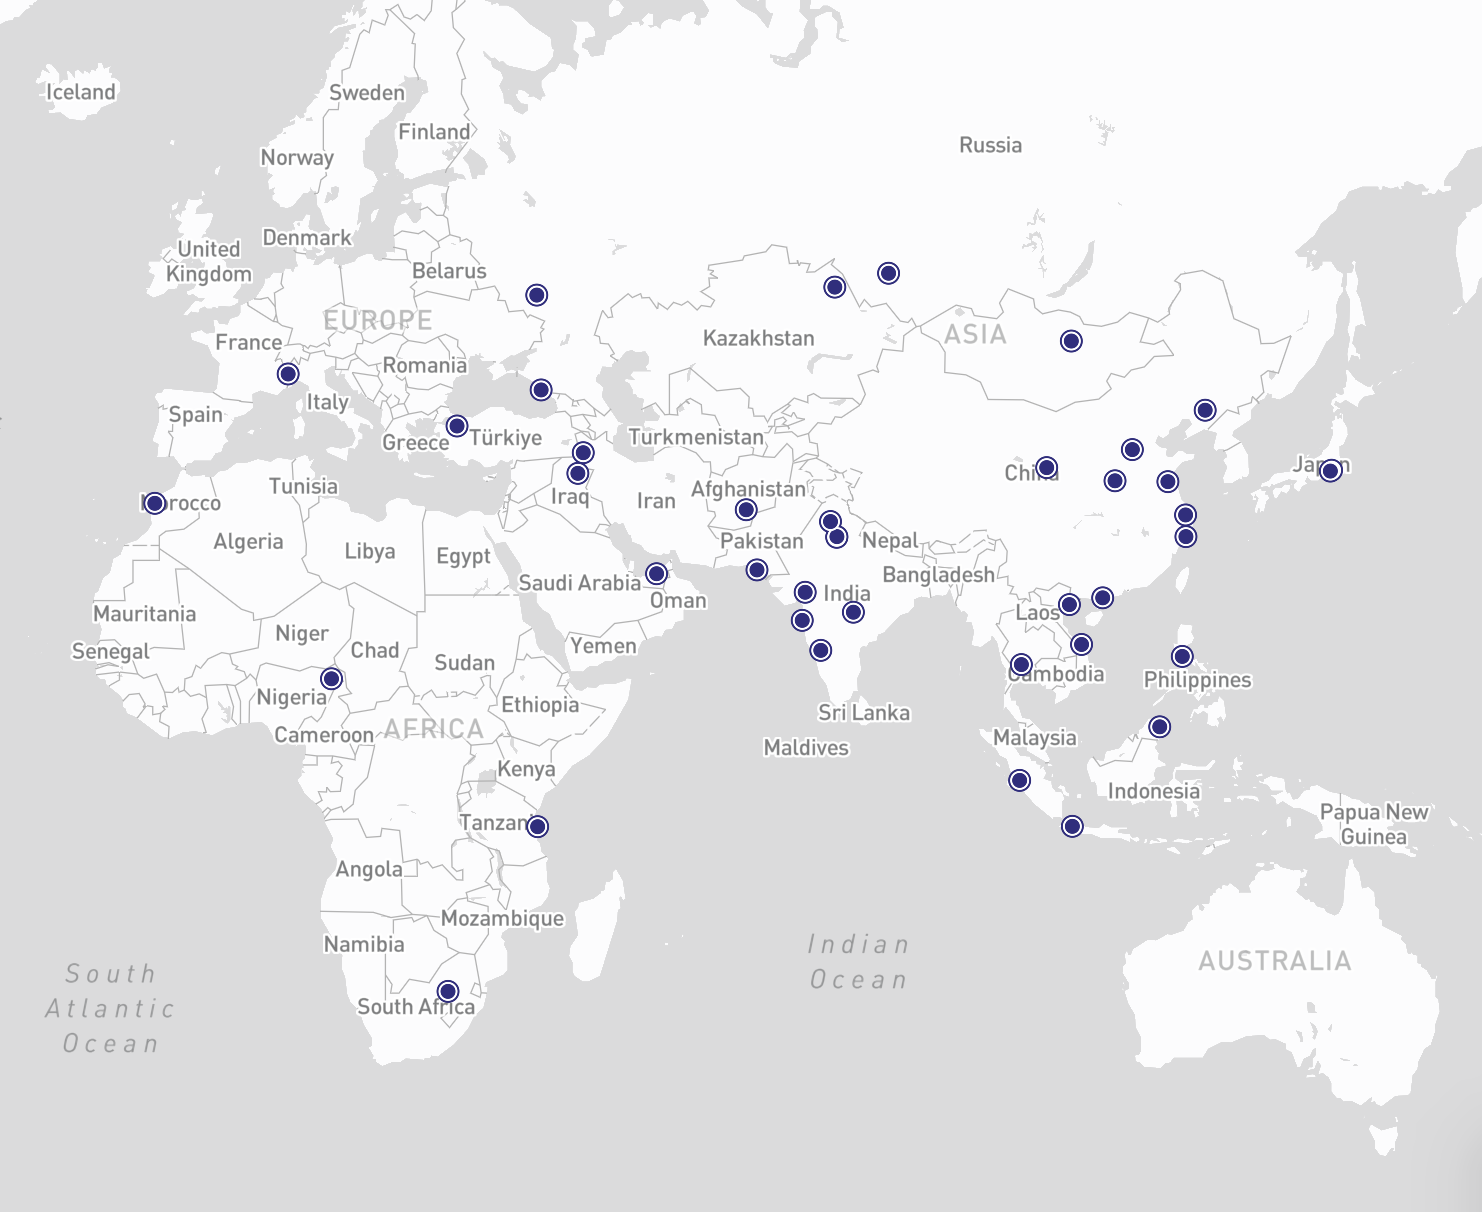
\includegraphics[width=\linewidth]{figures/40puntos.png}
    \caption{40 ciudades}
    \label{fig:mapa40}
\end{figure}

Sólo fue necesario ajustar de forma proporcional aquellos hiperparámetros dependientes del tamaño de la
entrada: el tamaño del lote (\texttt{batch}), el número máximo de intentos (\texttt{maxAttempts}) y la
muestra de temperatura (\texttt{tempSample}). Tomando como referencia los promedios calculados para la
instancia de 150 ciudades, la configuración escalada quedó definida así:
\begin{verbatim}
    -seed 19
    -targetP 0.8248
    -epsilonP 0.00001
    -initialT 8
    -tempSample 1600
    -coolingFactor 0.95
    -epsilon 0.00001
    -batchSize 1600
    -maxAttempts 42
\end{verbatim}

Para evaluar el desempeño en esta nueva instancia, se realizaron solo 100 ejecuciones independientes.
Mantuvo el $100\%$ de factibilidad y logró converger a la solución óptima de 0.2638195 en 25 de las
100 ejecuciones. Esta solución fue verificada con el registro histórico de cursos pasados. \\

La secuencia correspondiente a los identificadores de las 40 ciudades que conforman esta ruta
es la siguiente:

\begin{quote}
979, 493, 329, 163, 172, 496, 815, 657, 168, 1, 656, 2, 653, 490, 654, 7, 816, 982, 332, 820, 981, 333, 3, 165, 6, 5, 978, 817, 4, 489, 492, 491, 984, 331, 164, 327, 980, 244, 75, 652.
\end{quote}


\begin{figure}[H]
    \centering
    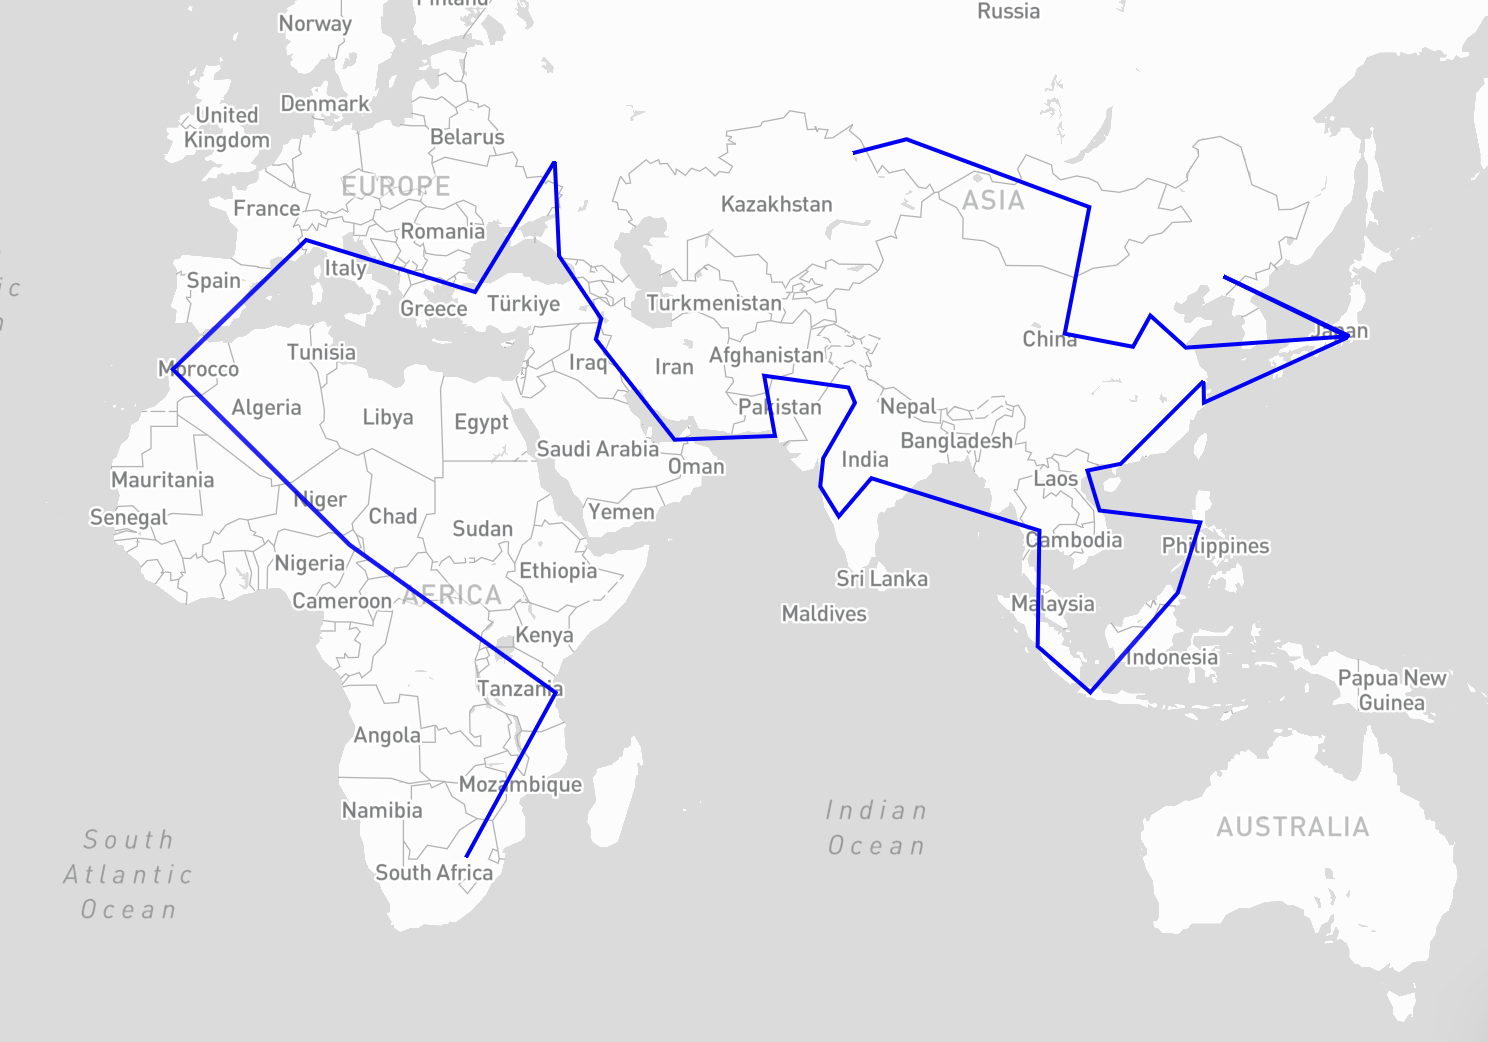
\includegraphics[width=\linewidth]{figures/Sol40_map.png}
    \caption{Ruta final obtenida por el algoritmo de Recocido Simulado para la instancia de 40 ciudades con costo 0.2638195}
    \label{fig:mapa40_sol}
\end{figure}

\begin{figure}[htbp]
    \centering
    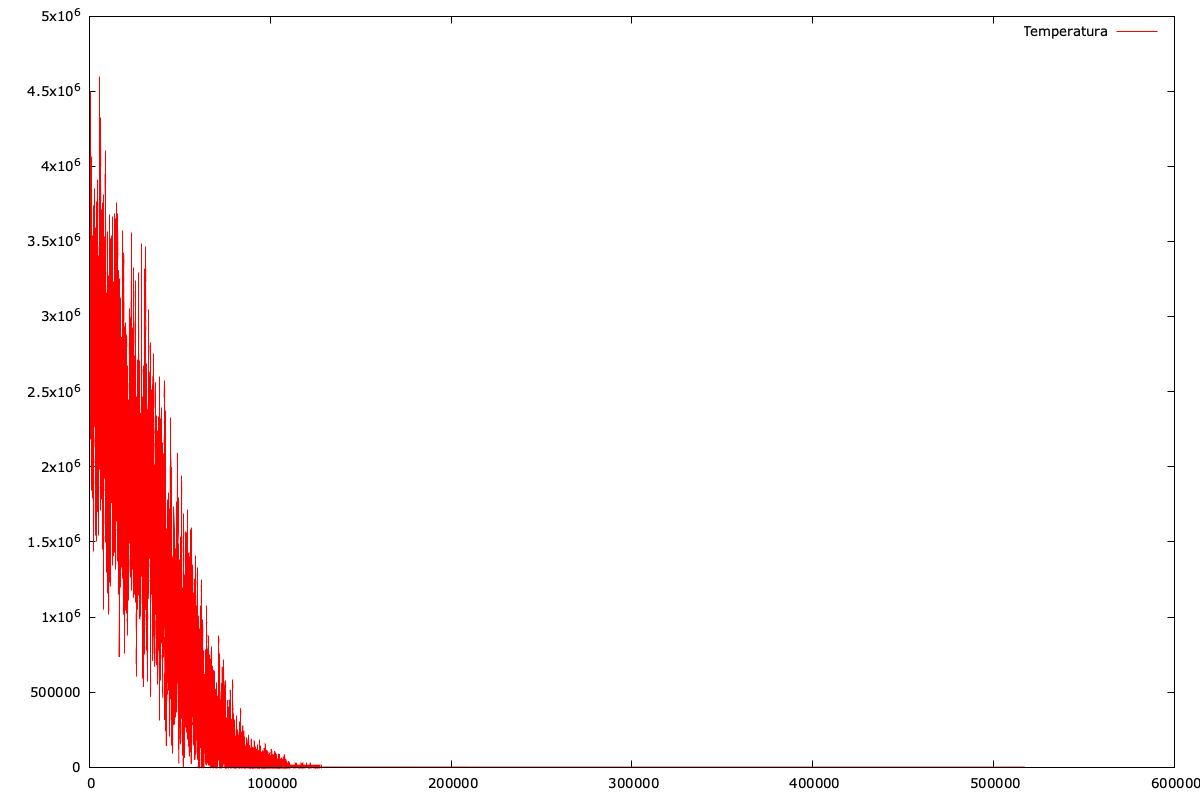
\includegraphics[width=\linewidth]{figures/acep40_1.png}
    \caption{Evolución de la función de costo con respecto a la temperatura en la ejecución de costo 0.2638195}
    \label{fig:acep40}
\end{figure}


\section{Dificultades y Limitaciones}
El desarrollo e implementación de este sistema presentó diversos retos de ingeniería de software y de
gestión de la experimentación. Por un lado, por una deuda técnica adquirida en las etapas tempranas del
desarrollo, no se tradujeron los identificadores originales de la base de datos al momento de generar
los resultados y en consecuencia las rutas en los archivos CSV requieren un procedimiento externo para
recuperar el contexto original de los datos. El mapeo es simple y puede usarse la clase
\texttt{EnvironmentTSP} con las instancias de la entrada para hacer la traducción.\\

Por otra parte, en las primeras fases del proyecto la carencia de un módulo de experimentación derivó
en la pérdida de información. Al no haber parametrizado los nombres de los archivos de salida, hubo
múltiples ejecuciones que sobrescribieron los reportes previos. Dolorosamente, se perdieron cerca de
20,000 ejecuciones cuyos resultados no se reportaron aquí, no fue posible recuperar los datos. También
hubo inconvenientes en etapas más avanzadas de la experimentación: al generar parámetros aleatorios con
una alta cantidad de decimales, el formato utilizado para guardar los registros en los archivos CSV
truncaba las cifras. Esta pérdida de precisión fue catastrófica para la reproducción exacta de algunas
de las mejores soluciones tempranas. Esto se resolvió limitando el número de decimales en los
hiperparámetros y formateando a 10 decimales en los archivos CSV.

\section{Conclusiones}
El sistema de Aceptación por Umbrales implementado logró resolver satisfactoriamente ambas instancias
del problema. Para la instancia de 150 ciudades, el algoritmo alcanzó un costo mínimo de 0.13624,
resultado reproducido de manera consistente por al menos 17 semillas distintas bajo la configuración de
hiperparámetros aleatorios de la tercera etapa y con un índice de máxima factibilidad. Para la instancia
de 40 ciudades, con la configuración promedio escalada al tamaño de la entrada, el sistema convergió
a la solución óptima de 0.2638195 en una cuarta parte de las ejecuciones, manteniendo también la
factibilidad del \(100\%\).\\

Lo más destacado del experimento fue cambiar el modelo de vecindad del intercambio simple de ciudades a
la inversión de subsegmentos. Esto permitió romper el estancamiento cerca del 0.14 al conservar mejor la
estructura de las rutas casi óptimas. Aunque el trabajo fue individual, comparar métricas con compañeros
que resolvían el mismo problema fue fundamental: esto impulsó la mejora y me motivó a compartir el
hallazgo con ellos. \\

Aún con estos resultados, no perfectos pero suficientemente buenos, el análisis de rendimiento revela 
un patrón de estancamiento: el algoritmo alcanza la solución 
convergente en torno al \(20\%\) del proceso y dedica el tiempo restante a una exploración que 
no produce mejoras significativas. Identificar la causa exacta de este comportamiento y más importante
aún, cómo mejorarlo, queda fuera del alcance de este proyecto por cuestiones de tiempo. %Siempre quise escribir eso :')

%----------------------------------------------------------
% Bibliografía
%----------------------------------------------------------

\printbibliography


\end{document}